\documentclass[11pt,twocolumn]{article}

\usepackage[a4paper, top=3cm, bottom=3cm, left=2.6cm, right=2.6cm]{geometry}
\usepackage{titlesec}
\usepackage{amssymb, amsmath}
\usepackage{color}
\usepackage{graphicx}
\usepackage{tabularx}
\usepackage[font=normalsize,skip=0pt]{caption}
\usepackage{floatrow}
\usepackage{wrapfig}
\usepackage{overpic}
\usepackage{booktabs}
\usepackage{caption}

\parskip 0pt   
%\titlespacing\section{0em}{0em plus 4pt minus 1pt}{0.2em plus 2pt minus 1pt}
%\titlespacing\subsection{0pt}{0em plus 4pt minus 1pt}{0.2em plus 2pt minus 1pt}
%\titlespacing\subsubsection{0pt}{0.5em plus 1pt minus 1pt}{0.1em plus 0pt minus 0pt}
\titlespacing\paragraph{0pt}{-0.064em plus 0pt minus 0pt}{1em plus 0pt minus 0pt}

\captionsetup{labelfont=bf}

%\titleformat{\section}
  %{\normalfont\normalsize\bfseries}{\thesection}{1em}{}

%SUBSECTIONS MUST BE IN NON-BOLD ITALIC

\setlength{\columnsep}{1 em}

\linespread{0.94}

\begin{document}
\title{AS03 Investigating the Merger-Free Co-Evolution of Black Holes}

%\author{564428}
\date{}

\twocolumn[
  \begin{@twocolumnfalse}
\vspace{-3em}

Supervisor: Dr. Brooke Simmons, and Dr. Chris Lintott\\
Candidate number: 564428\\
Word Count: 5913\\
    \maketitle

\vspace{-5em}

\renewcommand{\abstractname}{\normalsize Abstract}
    \begin{abstract}
\normalsize
%Here the structure is pretty good but a sentence of context at the start is a good idea, so that people know immediately why they should care. Here it would be something about how it is becoming increasingly clear that supermassive black hole growth in the absence of mergers is potentially a significant contributor to the overall growth of black holes, but that its effects on black hole-galaxy co-evolution are as yet unknown.
\noindent
 It is becoming increasingly clear that significant growth of supermassive black holes (SMBHs) is possible in the absence of galaxy mergers. However, the effects of this merger-free black hole growth on galaxy-black hole co-evolution are as yet unknown. To this end, I study a candidate sample of 26 visually selected bulgeless SMBH host galaxies, since a merger-free history manifests itself in a bulgeless morphology. Of this sample, parametric morophological fitting confirms that 24 of these galaxies show no sign of mergers, with 13 containing a non-merger driven pseudo-bulge contribution of  $>15 \%$, and 11 bulge contributions of $<15\%$. Out of these 24, X-ray data indicate that 15 objects host confirmed SMBHs, the other 8 are potentially star formation galaxies.  The existence of at least 15 (and possibly 24) mergerless SMBH hosts results supports earlier findings that significant BH growth is compatible with mergerless evolution and confirms this result to higher redshifts (up to $ z\sim1$). Furthermore, mass relations between $M_{BH}$ and $M_{host}$, and $M_{BH}$ and pseudo-bulge $M_{bulge}$, are consistent with established relations for merger-dominated classical bugles and elliptical galaxies, suggesting that mergers need not be fundamental to galaxy black-hole coevolution. Additionally, I observe a tentative increase of $M_{BH}/M_{bulge}$ with decreasing redshift, which agrees with earlier results for $z\sim 0$. 

%To this end this project aims to investigate the relation between supermassive black holes, and host galaxies that show no clear sign of merger. As a mergerless history manifests itself in a bulgeless morphology, {\color{red} Sample selection}   Furthermore, correlations between black hole and both disk and bulge mass are consistent with established relations for classical bulges and elliptical galaxies.

% implies a merger-free history

%   It is becoming increasingly clear that significant growth of supermassive black holes (SMBHs) in the absence of galaxy mergers is potentially a significant process.
% 

%Therefore, in order to investigate the processes driving the growth of SMBH black holes I investigated a sample of 26 bulgeless AGN hosts.  

%This suggests that merger-free, secular processes can contribute significantly to black hole growth.

% Parametric morphological fitting indicates that 25 of the galaxies in the sample are indeed mostly bulgeless, while X-ray data indicate that they host significant SMBHs.

% If, therefore, it would be possible to locate a sizeable and secure sample of bulgeless galaxies hosting SMBHs, this would form a strong argument that SMBH formation can occur through mergerless processes. In fact, such a sample has already been presented by Simmons et al \cite{Simmons01032013}. The main object of this project is to expand this sample, and extend the study of merger-free black hole growth to higher redshift (up to $\sim z=1$), which has the additional advantage of enabling investigation of black hole growth over a longer time scale. 
%\par The sample of galaxies has been obtained from Hubble Space Telescope images, which have been classified by Galaxy Zoo as (largely) bulgeless, with the additional requirement that they host an active galactic nucleus (AGN). The sample presented here contains 25 such galaxies, with images in the I band and V band. The program {\tt GALFIT}  \cite{Peng:2009fu} was used to perform parametric morphological fitting to resolve the image into its components: disk, bulge and AGN. From this decomposition, an upper limit on the classical bulge mass can be obtained by comparing the contribution of the bulge and the disk luminosities, and a more secure conclusion can be reached as to whether these galaxies are indeed (largely) bulgeless. Finally, black hole masses are compared to  their host galaxy masses and (upper limits on the) classical bulge masses, in order to investigate whether these mergerless galaxies follow the same galaxy-black hole mass relation as elliptical and bulge-dominated galaxies with a clear history of mergers. If it is indeed shown that the mergerless galaxies follow the same disk mass-black hole mass relations as the galaxies that have undergone mergers, this might imply that the merger history of galaxies is not fundamental to the co-evolution of galaxies and their SMBHs.  
\vspace{1em}
    \end{abstract}
  \end{@twocolumnfalse}
]

\section{\normalsize INTRODUCTION}\label{intro}

%The influence of mergers on the evolution of galaxies, and the role of supermassive black holes in this process, is one of the central issues in modern galaxy evolution theory.

One of the central topics in modern galaxy evolution theory concerns the influence of mergers on the evolution of galaxies, and the role of supermassive black holes in this process. According to the predominant paradigm,  mergers are believed to form galaxies hierarchically, driving the growth of SMBHs in this process \cite{1988ApJ...325...74S} \cite{2008ApJS..175..356H} \cite{2006MNRAS.365...11C}. However, an increasing body of evidence suggests that mergers are not required to grow a central black hole at any $z< 3$ \cite{2011ApJ...727L..31S} \cite{2012ApJ...744..148K} \cite{2012ApJ...761...75S} \cite{Simmons01032013}. In order to quantify the effect of such merger-free processes on black hole growth, a sample of SMBHs in galaxies with no history of mergers will be required. 
\paragraph{} This evolutionary history can partially be traced through a galaxy's morphology \cite{1987gady.book.....B}. For instance, spiral galaxies are dynamically cold systems, consisting of a disk of stars and interstellar medium, rotating fairly uniformly around the galactic centre. Elliptical galaxies on the other hand, are dynamically hot with stellar motions unordered, and have a steeper density profile than disks. Major mergers between spiral galaxies are known to result in ellipticals. Physically, when two rotating disks approach each other at an angle, gravitational interactions will violently mix up the stars and destroy the uniform disk motions, resulting in an elliptically shaped galaxy with randomly distributed stellar motions.  Similarly, minor mergers of a larger disk galaxy with a smaller companion invariably produce a central elliptical component called a bulge . Thus, as a bulgeless morphology implies an evolutionary history free of mergers and other violent processes.

%, this project concentrates on bulgeless galaxies. 
% {\color{red} mention ellipticals are no longer forming stars?}.
\paragraph{}Most (if not all) galaxies host a central supermassive black hole (SMBH, $ m_{BH} \gtrsim 10^6 M_{\odot}$) \cite{1998AJ....115.2285M} \cite{2004MNRAS.351..169M}. Active galactic nuclei (AGN) are unusually bright regions in the centres of galaxies, believed to consist of radiation emitted by such an accreting SMBH \cite{1969Natur.223..690L}\cite{1989ApJ...340L...5C}. Their exceptional brightness allows them to be clearly visible even in bright galactic centres, providing a means of SMBH detection as well as a handle on properties such as BH mass. It is often claimed that central SMBHs have accumulated their sizeable masses from galaxy mergers, either through merging with other galaxies' SMBHs, or through additional accretion fueled by violent disruption of galactic matter in the merger process. In support of this hypothesis, strong correlations exist between black hole mass and bulge properties \cite{2000ApJ...539L..13G}\cite{1998AJ....115.2285M}\cite{2003ApJ...589L..21M}\cite{Haring:2004hr}, suggesting close co-evolution in the case of these merger-dominated objects.
\paragraph{} However, in light of the aforementioned recent suggestions of merger-free black hole growth, I aim to investigate whether similar galaxy-black hole relations exist in a sample of mergerless galaxies. A sample of such bulgeless merger-free AGN hosts has previously been identified by Simmons et al. 2013 \cite{Simmons01032013} for $z\sim 0$. In this project I expand on this sample, presenting 26 bulgeless AGN host candidates, and extend the depth up to higher redshifts of $ z\sim 1$. This corresponds to a time when the universe was around 6 Gyr old, allowing for the study of merger-free black hole growth over a longer period of cosmic time. 
\paragraph{} Section \ref{data} describes the imaging and selection of the candidate sample and data, as well as X-ray AGN selection. Section \ref{fitting} describes methods used in this project, and in particular the process of parametric morphological fitting. In Section \ref{results} I present the results of this process, and in Section \ref{mass}, I explain how I obtained galaxy and black hole masses. Section \ref{discussion} explores the implications of the results of this project for galaxy black hole co-evolution. Throughout this project, I have assumed $H_{0} = 71$  km s$^{-1}$ Mpc$^{-1}$, $\Omega_{M} = 0.27$ and $\Omega_{\Lambda} = 0.73$, to retain consistency with earlier data used in this project. 
\paragraph{}

%{\color{red} Goals: BH-galaxy relations. z=0 by Simmons et al.}
%\subsection{\normalsize Galaxy Morphology}
%Explain about different types of galaxy, and mainly about bulges (and pseudo-bulges). Also explain about AGN and that they are believed to be caused by an accreting SMBH. 
%\subsection{\normalsize The Role of Mergers in Galaxy Evolution}
%Explain that mergers are believed to produce bulges and quickly explain the physical mechanism through which this happens (disks with angular  momentum approach each other at an angle, gravitational interactions/conservation of AM scrambles up the stars producing a bulge). It is also thought that SMBHs grow to their supermassive ($\sim10^6$ solar masses?) size through mergers (READ MORE AND SUPPORT THIS STATEMENT WITH REFERENCES). However, Simmons et al \cite{Simmons01032013} found a sample of mergerless galaxies hosting AGN. These galaxies did not obey the BH-Bulge relation from H\"{a}ring and Rix (cite). Furthermore the data were consistent with the BH disk-relation of Elliptical galaxies (with a clear history of mergers), implying that mergers may not be crucial to BH-galaxy coevolution. One sentence explaining whether my research agrees with/adds to this. 

\section{\normalsize IMAGE AND DATA SELECTION}\label{data}
\subsection{\normalsize Data}
\subsubsection{\normalsize Optical AGN and Host Galaxy Imaging}
Reliable bulge-disk and point-source decomposition of AGN host galaxies at redshifts $z \gtrsim 0.1$ requires deep space-based observations in a field with excellent multi-wavelength data for selection of AGN. This project thus uses images taken from the Great Observatories Origins Deep Survey (GOODS) \cite{2003mglh.conf..324D} with the Advanced Camera for Surveys (ACS) on the \emph{Hubble Space Telescope (HST)}. The survey covered roughly 320 square arcminutes in two fields, centered on the \emph{Hubble} Deep Field North (HDF-N) and the \emph{Chandra} Deep Field South (CDF-S) \cite{2004ApJ...600L..93G}. Observations encompass optical and near-infrared imaging in the F435W, F606W, F775W, and F850LP passbands, also referred to as $B$, $V$, $I$, and $z^\prime$. 
%{\color{red} Talk about image selection} 
\paragraph{}  In order to  maximise any possible bulge flux, it is generally preferable to use the reddest available imaging, as classical bulges are no longer forming stars and thus contain redder stellar populations \cite{2004ARA&A..42..603K}. However, because the reddest ACS $z^\prime$-band  has higher background noise and a noisier PSF (for PSF see Section \ref{psf}), this project focuses on the next reddest, i.e. $I$-band imaging.
%From these observations, galaxies were identified, cut out at each available wavelenth, and combined into colour images by Roger Griffith using GALAPAGOS \cite{2011ASPC..442..155H}.

%\paragraph{} The images that include galaxies were subsequently incorporated into the Galaxy Zoo project\cite{bla}, and classified by citizen scientist volunteers. On www.galaxyzoo.org Galaxy Zoo volunteers were asked to classify objects randomly selected from the aforementioned sample of galaxies by clicking buttons in response to questions describing the galaxies' morphology. The images used in this project have been selected to have been classified by at least xxx people as bla. 

\subsubsection{\normalsize X-ray data}
X-ray data in the soft (0.5 - 2 keV) and hard (2 - 8 keV) bands were taken from the \emph{Chandra} point-source catalogs of Alexander et al. \cite{2003AJ....126..539A} and Xue et al. \cite{2011ApJS..195...10X} for the HDF-N and CDF-S, respectively. These  fields contain some of the deepest X-ray observations, at 2 Ms and 4 Ms respectively, providing more than adequate depth to detect AGN emission at all redshifts considered in this project. 
\paragraph{} The  X-ray point sources were matched to optical sources by Cardamone et al. 2008 \cite{2008ApJ...680..130C} and Bauer et al. 2002 \cite{2002AJ....124.2351B}, 2004 \cite{2004AJ....128.2048B} using a maximum likelihood algorithm. 

%Also, it's worth mentioning somewhere that the X-ray sources were matched to the optical sources via a maximum likelihood method (Cardamone et al. 2008; Bauer et al. 2002, 2004).  (These are the people I got the matches from, and they published some details the method in these papers.)

\subsubsection{\normalsize Redshifts}
The analyses in this project require reliable distance measurements in the form of spectroscopic redshifts. Redshifts used in this project were obtained from  Wirth et al. 2004 \cite{2004AJ....127.3121W}, Cowie et al. 2004 \cite{2004AJ....127.3137C}  and Barger et al \cite{2008ApJ...689..687B}. 
%of the spectroscopic redshifts, refer to Barger et al. (2008)

%For z origin equal to GOODS-N-ALL, refer
%to Wirth et al. (2004) and Cowie et al. (2004); for the remainder
%of the spectroscopic redshifts, refer to Barger et al. (2008)


%You need another subsection here for ancillary data: In particular, you need to discuss redshifts. The redshifts are collected from many sources and you just need to give each of them credit and note that all the redshifts used here are spectroscopic. The redshift sources should be mentioned in Griffith et al., Alexander et al (maybe), and Xue et al, and they may include e.g. Szokoly et al. (2001, I think, but not sure).

%The X-ray data for the HDF-N were taken from Alexander et al 2003 \cite{2003AJ....126..539A}, who identified point sources in the  2 Ms Chandra Deep Field-North survey. A portion of this field is also covered by the GOODS HDF-N, allowing the sample of bulgeless galaxies to be narrowed down to those objects containing point sources. For the southern part of the sky, point source catalogs were obtained from Xue et al 2011 \cite{2011ApJS..195...10X}, which covered the CDF-S. The data from both surveys contain X-ray emission in the hard band (2-8 keV) and soft band (0.5-2 keV).

%Rewrite this to something like: X-ray data in the soft (0.5 - 2 keV) and hard (2 - 8 keV) bands were taken from the \emph{Chandra} point-source catalogs of Alexander et al. (2003) and Xue et al. (2011) for the HDF-N and CDF-S, respectively. These are two of the deepest X-ray fields, at 2 Ms and 4 Ms, respectively, with more than adequate depth to detect emission from a SMBH at all redshifts considered in this report.


%\paragraph{}It must be noted however, that these point sources need not necessarily originate from AGN, as star formation or X-ray binaries can sometimes produce similar X-ray point source emission. The problem of determining which galaxies host significant AGN will be addressed in section \ref{xray}. 

\subsection{Sample selection}
\subsubsection{Visual inspection}
The sample of candidate bulgeless consists of 26 AGN host galaxies, and was selected by B. Simmons after visual inspection of 288 optical matches to X-ray point sources. The 26 candidate colour images are displayed in Figure \ref{mosaic}. As explained in Section \ref{results}, objects 50006849 and 90044623 were rejected from the sample. From visual inspection it is evident that galaxy orientations vary from face-on to nearly edge-on, and span a range of colours.  Additionally, the sample contains both barred and unbarred disks and a variation in tightness of spiral windings. Thus, the analysis presented in this project should contain no significant bias towards a particular type of disk morphology. 

\begin{figure*}[!t]
%\centering
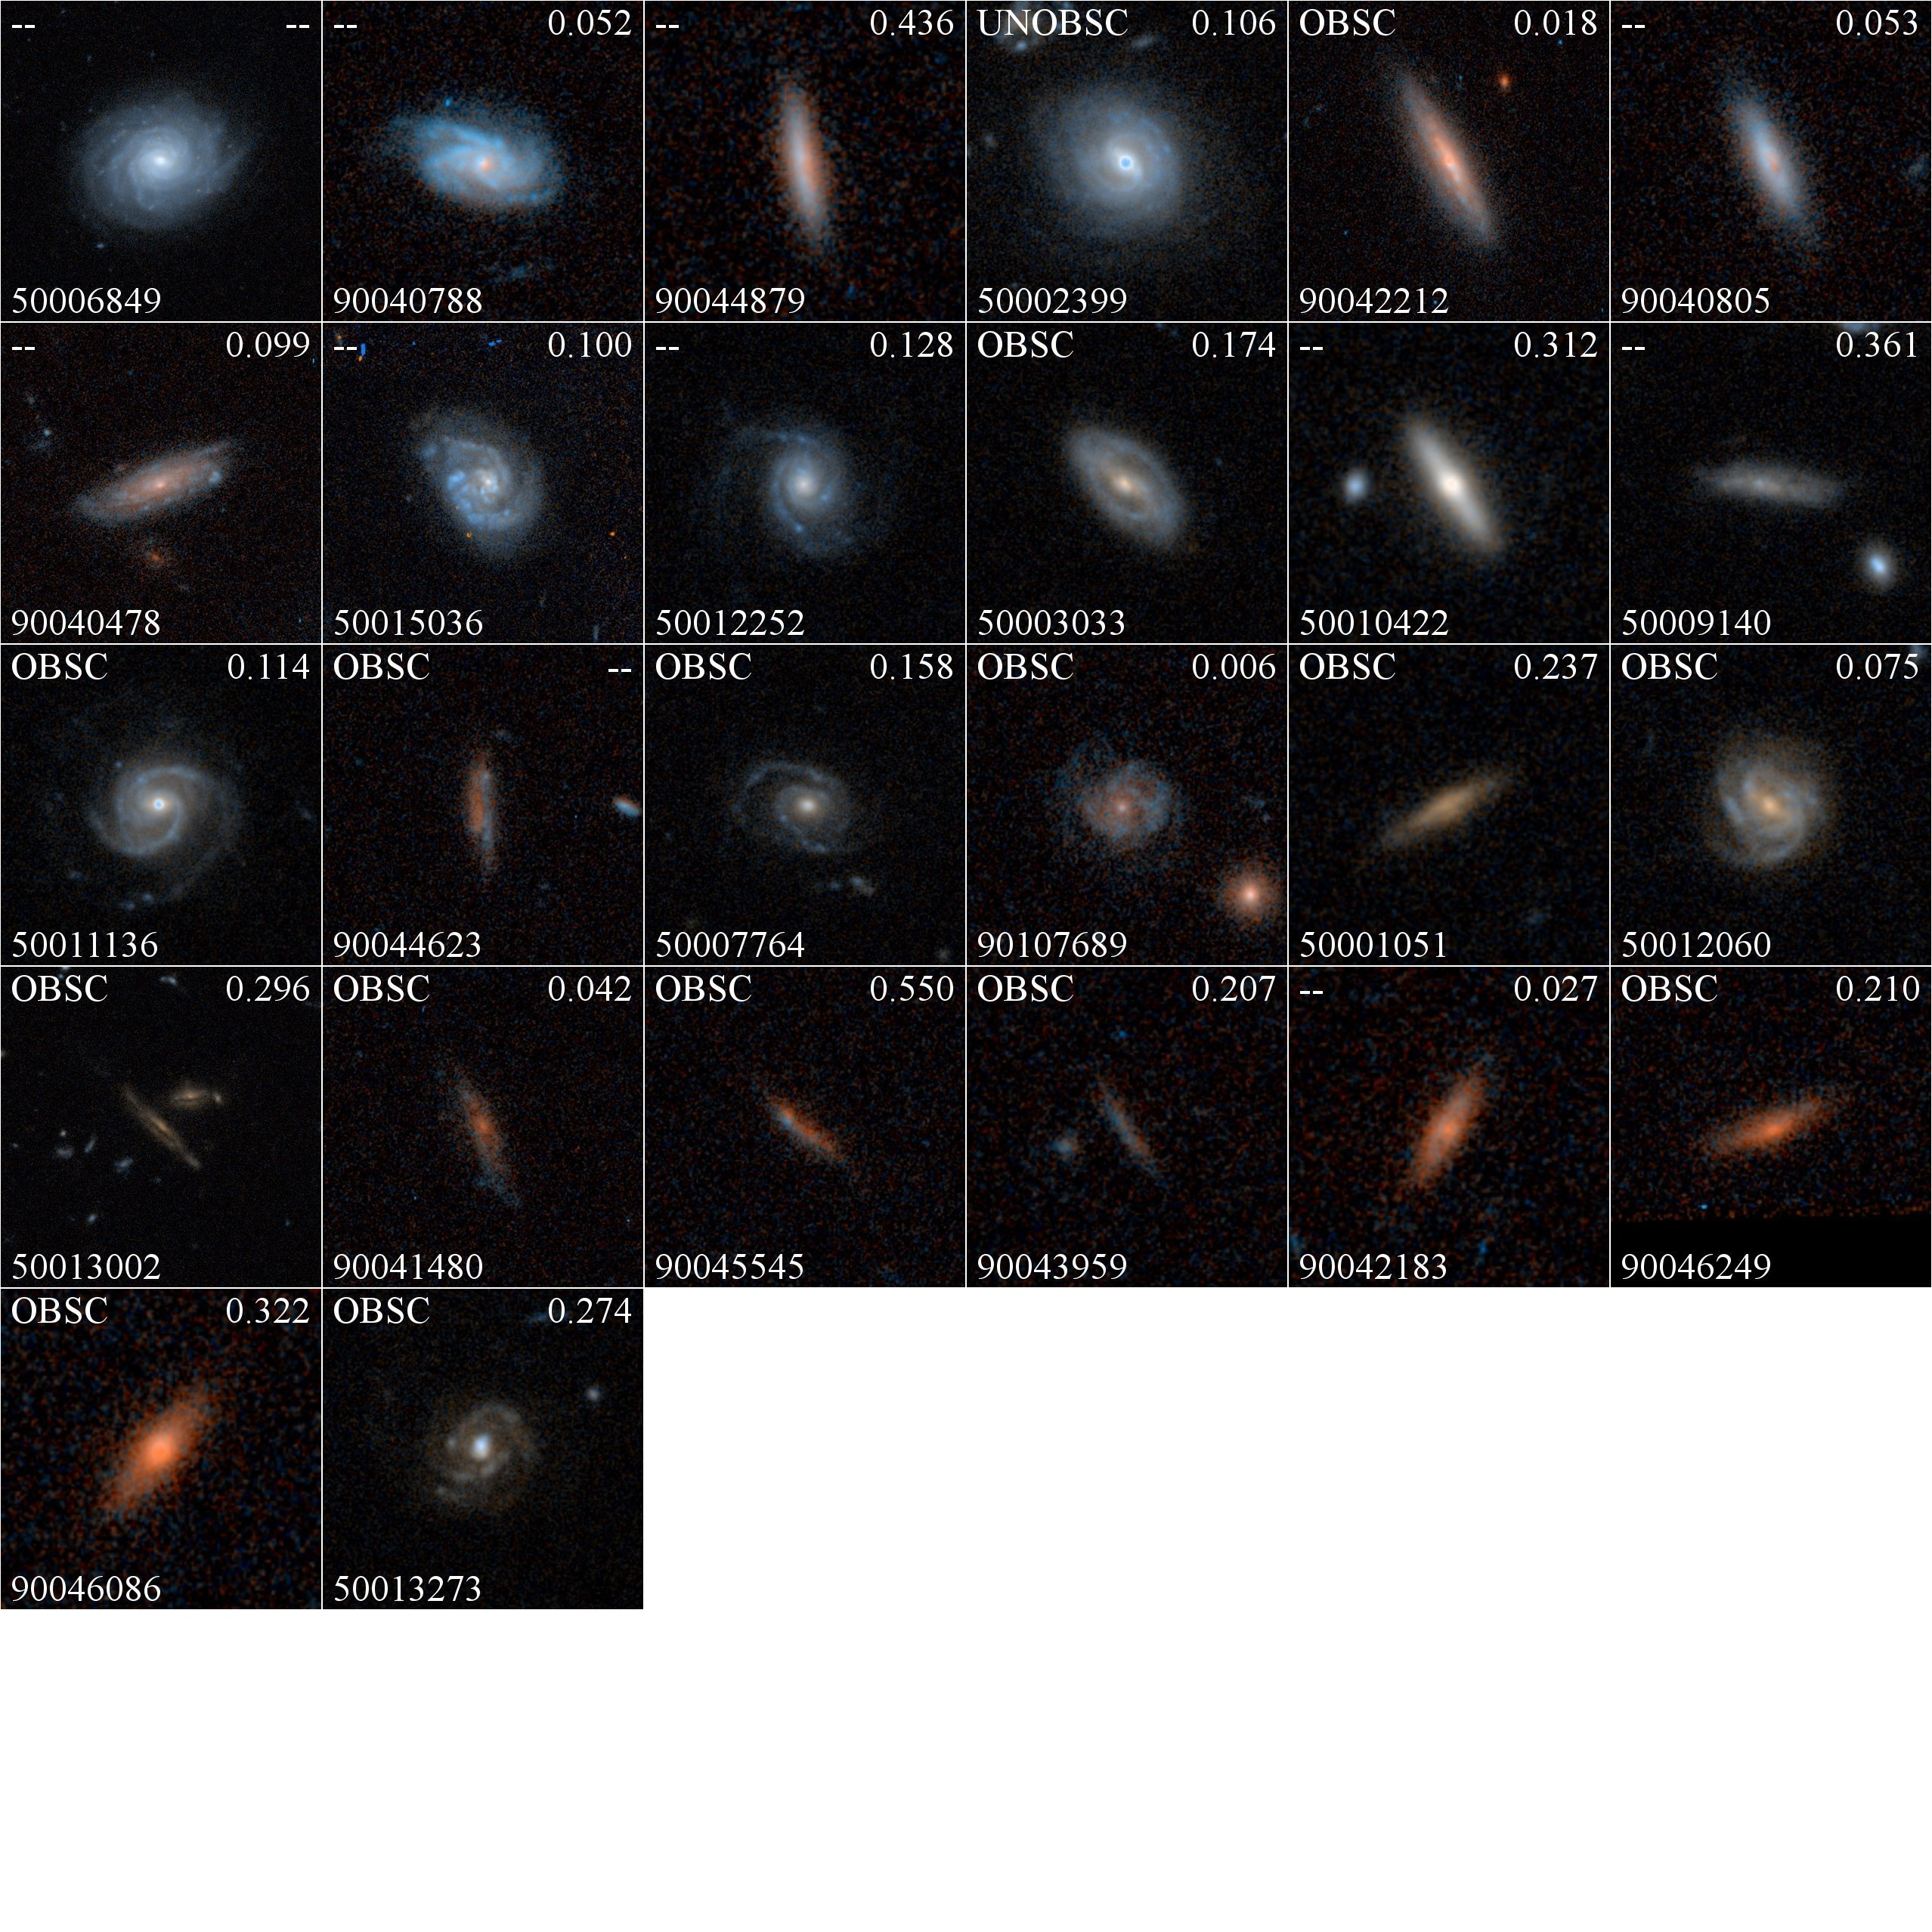
\includegraphics[width=\textwidth]{Mosaic2}
\caption{ Galaxy Zoo \cite{2013MSAIS..25...82M} colour images of 26 candidate bulgeless AGN hosts, sorted by ascending redshifts. AGN classifications, and bulge-to-disk luminosity ratios are inscribed in the top left and top right corner respectively. Object 50006849 contains a classical bulge and 90044623 could not be decomposed by parametric fitting. Both were removed from the sample. Of the remaining 24 galaxies, 15 objects contain X-ray confirmed obscured (OBSC) or unobscured (UNOBSC) AGN. 13 contain pseudo-bulge contributions of $>15\%$, the other 11 are predominantly bulgeless, indicating that all 24 galaxies have a merger-free history.}
\label{mosaic}
\vspace{-7em}
\end{figure*}
\vspace{-1em}

% Visual selection was based on colour images from Galaxy Zoo: Hubble (Melvin et al. 2013), but did not use volunteer classifications from that project owing to the tendency of AGN emission to bias volunteer classifications (Section \ref{agnbias}). 

\subsection{AGN selection} 
In addition to AGN activity, star formation and X-ray binaries can also contribute to X-ray flux. In order to reject galaxies where these processes dominate X-ray emission, I clasified objects according to their hard band X-ray luminosity and hardness ratios ($ HR =  \frac{H -S}{H+S}$, where $H$ and $S$ are the net count rates in the hard  and soft band). Throughout the project I employed the following selection criteria, based on criteria in Szokoly et al 2004 \cite{2004ApJS..155..271S}:
%

\begin{itemize}
\item{\textbf{Unobscured AGN}: hard X-ray luminosity $L_{x} > 10^{42}$ erg/s and $HR \leq -0.2$} 
\item{\textbf{Obscured AGN}: hard X-ray luminosity $L_{x} > 10^{41}$ erg/s and $HR > -0.2$}
\end{itemize}

Object 50002399 contains an unobscured AGN, and 14 others contain obscured AGN. The other 9 fall outside these categories. However, the faint flux limit of the deep X-ray images means that not all galaxies are expected to show clear indications of AGN activity from the X-ray emission alone. Parametric morphological fitting detects significant point sources for all 9 objects that fall outside the above selection criteria (see Table \ref{resulttable}). As spurious point source detection in parametric fitting is fairly uncommon (e.g. Simmons \& Urry 2008 \cite{2008ApJ...683..644S} finds a maximum rate of 25 \% in bulge-dominated sources), these 9 galaxies are retained in the sample of bulgeless AGN hosts, and shall be classified as ``uncertain AGN". All classifications are displayed in Figure \ref{mosaic}. 

% L_X > 1e42 and a hardness ratio of <= -0.2, and an obscured AGN will have L_X > 1e41 and HR >= -0.2

%{\color{red} Talk about the final sample}

%The faint flux limit of the deep X-ray images means that only a fraction of the 26 candidate bulgeless AGN are expected to show clear indications of AGN activity from the X-ray emission alone. 
%(Then describe the X-ray criteria and how you select unambiguous obscured and unobscured AGN from the X-ray luminosities and hardness ratios. GIve numbers of each. Then say that for the remainder you use the results of point-source/host galaxy decomposition to determine whether nuclear emission is likely or ruled out, and refer readers to later sections where you discuss the fitting and results of.



%Additionally, spectroscopic redshifts obtained from GOODS indicate a redshift range of between z=0.137 and z=0.9712.

% 
%(Then describe the X-ray criteria and how you select unambiguous obscured and unobscured AGN from the X-ray luminosities and hardness ratios. GIve numbers of each. Then say that for the remainder you use the results of point-source/host galaxy decomposition to determine whether nuclear emission is likely or ruled out, and refer readers to later sections where you discuss the fitting and results of.

%Then, "Colour images of all 26 candidate bulgeless AGN and host galaxies are displayed in Figure…"


%\paragraph{} It must  be born in mind that the sample presented in this project was selected with an emphasis on being securely bulgeless and active, rather than representative. Future work would be needed to investigate how common bulgeless active galaxies are among the total population. MOVE TO LATER, talk about automated fitting (though explain the need for visual classification, as bulges can be way off). 

%In this project parametric morphological fitting was performed on from V band (visual) and i band (near infrared) images, also provided by Brooke Simmons. 


%To find the masses of the BH we used X-ray data (explain why, less obfuscation by dust, better understood relation to Bolometric luminosity?). Mention where these data came (Chandra X-ray observatory with hard band: 2-8 keV, soft band: 2-8 keV, and the infrared magnitudes are from WISE with wavelenghts 3.3526, 4.6028, 11.5608, 22.0883 microns).

%\subsection{AGN}
%AGN are X-ray selected sources. It is also important to note that AGN can visually mimic central bulges, making it harder determine whether a galaxy is truly bulgeless, as well as obfuscating what contribution is due to a small bulge. This is one of the reasons why parametric morphological fitting is particularly important, as it allows one to resolve contributions from the disk, bulge and AGN, allowing a more precise determination of whether a galaxy is truly bulgeless (and if not, to find an upper limit on the size of its bulge). 
%\paragraph{}The sample of galaxies has been selected by my supervisor through matching galaxies with an AGN to those classified by Galaxy Zoo as bulgeless. In Galaxy Zoo volunteers in the general public are asked to visually classify galaxies by answering questions regarding their shape and orientation. The relevant questions for the selection of this particular sample are mainly concerned with the prominence of the central bulge compared to the rest of the galaxy.
%\paragraph{} Explain about bulges and pseudo-bulges. 
%\paragraph{} An Active Galactic Nucleus (AGN) is a a compact region at the centre of a galaxy which emits a large amount of electromagnetic radiation, believed to be caused by accretion of mass onto a supermassive black hole. The AGN in our host galaxies have been identified by <some criterion>. 
%\paragraph{}It is important to point out that a bright AGN can visually mimic a central bulge, making it harder to determine whether a galaxy is truly bulgeless, as well as obfuscating the contribution of whatever small bulge might be present. This

\section{\normalsize METHODS AND FITTING\label{fitting}}
\subsection{\normalsize Methods}
A considerable part of this project involved parametric morphological fitting with {\tt GALFIT}.  I wrote scripts in bash in order to automate parts of this process, such as running {\tt GALFIT} automatically, and generating input files and catalogs. Some tasks regarding images, such as creating bad pixel masks, and image scaling, required use of {\tt IRAF} \cite{1993ASPC...52..173T}. Throughout this project, I used {\tt TOPCAT} \cite{2005ASPC..347...29T} for handling datasets, as well as for computing and converting  between astrophysical quantities. For the F-test described in Appendix\ref{ftest}, I created scripts in the R programming language \cite{Rprogramming}. The remainder of this Section presents the details of parametric morphological fitting. 


\subsection{\normalsize Motivation for parametric fitting}
\subsubsection{\normalsize AGN can visually mimic bulges}\label{agnbias}
As both AGN and bulges resemble an extended bright central region on the images, visual inspection may lead to an incorrect classification. Thus, in order to obtain a more certain measure of the presence of bulges or AGN, it is necessary to follow up this visual classification with a more secure way to separate AGN, disk and bulge. Additionally, a quantitative analysis will require measurements of bulge-to-total ratios. To this end, this project employs parametric morphological fitting of the candidate sample, to separate the AGN point source contribution from disks and spatially extended central bulges.

%For instance, morphological classification mainly leads to an overestimation of the bulge component, as demonstrated by Galaxy Zoo simulations  in Simmons et al. 2013 \cite{ Simmons01032013}.


% Therefore, as a strict selection of only objects that appear to have no bulge at all, might exclude many AGN host galaxies that are in actual fact bulgeless, broader selection criteria were employed.  %(of which a detailed description is offered in section 3) 

 \subsubsection{\normalsize Distinguishing between classical bulges and pseudo-bulges}\label{pseudo-bulge}
An important issue in the morphological classification of bulges concerns the distinction between bulges and pseudo-bulges. Classical bulges (sometimes simply called `bulges') have a similar light distribution profile and obey similar parameter correlations to elliptical galaxies. As mentioned in Section \ref{intro}, they are equally believed to result from minor mergers. Pseudo-bulges, on the other hand, have properties more akin to disks, including shallower light profiles than classical bulges (though often slightly steeper than disks, with typically $n \lesssim 2$). They are believed to be formed in internal processes such as relatively fast (but still cold) gas accretion, and from various strong disk instabilities such as bars and large-scale clumps. They are thus consistent with a merger-free history \cite{doi:10.1146/annurev-astro-082708-101811} \cite{2004ARA&A..42..603K}.  As such, pseudo-bulges are admissible in our mergerless sample, and the term `bulgeless' shall henceforth refer to galaxies lacking a classical bulge, but not necessarily a pseudo-bulge. 
\paragraph{} Parametric fitting of a S\'{e}rsic profile (see Section \ref{parfitting}) to a bulge can be used to distinguish classical bulges from pseudo-bulges. An exponential disk profile has S\'{e}rsic index $n=1$, whereas a de Vaucouleurs elliptical has $n=4$ \cite{Peng:2002ua}. It has been shown that almost all classical bulges have $n \geq 2$ \cite{2010ApJ...716..942F}, and although some pseudo-bulges might have $n \approx 4$, the $n<2$ criterion employed in this project  should be a reliable sufficient condition for characterising pseudo-bulges \cite{doi:10.1146/annurev-astro-082708-101811}. 

%Thus the $n$ values are closer to $1$ for the disk-like pseudo bulges, and closer to $4$ for the elliptical pseudo-bulges. 
%\paragraph{} {\color{red} When a pseudo-bulge was detected, its luminosity was considered an upper limit on the classical bulge luminosity, as any smaller classical bulge could have been left undetected due to the presence of this large pseudo-bulge. The luminosity ratio  $L_{bulge}/L_{galaxy}$ thus gives a quantitative indication of bulgelessness. }
%If parametric fitting would have indicated a significant classical bulge, this galaxy would have been discarded from the sample. However, w
%^^ there is room for deletion here%If parametric fitting indicates a pseudo-bulge, this shall be taken as an upper limit on the size of a possible classical bulge, as smallr classical bulgse could have been left undetected. $L_{bulge}/L_{disk}$ thus quantifies how bulgeless a galaxy is. 

\subsection{\normalsize Parametric morphological fitting using {\tt GALFIT}}
%We need Parametric morphological fitting to find Disk and Bulge luminosities, most importantly to find an upper limit on the bulge mass. It is important to note that AGN can visually mimic central bulges, making it harder determine whether a galaxy is truly bulgeless, as well as obfuscating what contribution is due to a small bulge. Parametric morphological fitting allows one to resolve contributions from the disk, bulge and AGN, allowing a more precise determination of whether a galaxy that has been identified as visually bulgeless is truly bulgeless (and if not, to find an upper limit on the size of its bulge). We might also need the disk luminosity to find disk masses (though I don't know yet how this will work). \\
Parametric morphological fitting was performed with {\tt GALFIT}, developed by Peng et al \cite{Peng:2002ua} \cite{Peng:2009fu}, which can simultaneously fit an arbitrary number of components to an image, including offset components such as companion galaxies. The user specifies initial guesses for these components, and {\tt GALFIT} will determine the best-fit parameters in an iterative procedure using a $\chi^2$ minimisation algorithm. 
\paragraph{} {\tt GALFIT} produces three output images, as well as a log file containing final fit parameters and uncertainties. An example of these is presented in Figure \ref{examplefigure} for object 50002399. The first output image is the original input image cut to the size of the fitting region, and the second image is the best fit model. The third image contains the ``residuals", i.e. the model subtracted from the first image. 
\paragraph{} Detailed modelling of spiral arms and bars was not required for the purposes of this project, so all components used in this project were axisymmetric and smooth. The following sections explain details of these components. 


\subsubsection{S\'{e}rsic profile}\label{parfitting}
The S\'{e}rsic light profile for fitting disks and bulges has the following functional form: 
\begin{equation}
\Sigma(r) = \Sigma_e \exp \left[ -\kappa \left( \left(  \frac{r}{r_e} \right)^{1/n} - 1 \right) \right]
\end{equation}
$\Sigma(r)$ gives the pixel surface brightness at radius $r$, and $\Sigma_e$ gives the pixel surface brightness at the effective radius $r_e$. The effective radius is defined such that half the flux falls within $r_e$. $n$ is the S\'{e}rsic index, and quantifies how concentrated the light distribution in the core is compared to that in the outer regions, with $n=1$ corresponding to an exponential disk, and $n=4$ to a de Vaucouleurs elliptical.\cite{Peng:2002ua} . Given these constraints from  $\Sigma_e$, $r_e$ and $n$, the value of $\kappa$ is fixed for a given $n$. {\tt GALFIT} can also fit S\'{e}rsic profiles at an angle to the direction of view. The S\'{e}rsic profile has been implemented with the following free parameters: position coordinates $x$ and $y$, integrated magnitude, effective radius, S\'{e}rsic index, axis ratio $(b/a)$, position angle. 
%^ALL IN ALL

\subsubsection{Point Spread Function (PSF) }\label{psf}
The point spread function (PSF) quantifies the response of the imaging system to a point source. {\tt GALFIT} requires a convolution PSF image provided by the user. The PSFs used in this project are empirical PSFs for each field (HDF-N and CDF-S) and band ($I$ and $V$), created by the GOODS team and based on $~\sim 30$ stars each.  {\tt GALFIT} requires 3 free parameters for the PSF: $x$ and $y$ coordinates, and total magnitude. 

% using the daophot routines in IRAF \cite{bla} 

\subsubsection{Background Sky}
The sky background allows the user to model either a fixed constant background value across the image, or to vary this value in both the $x$ and $y$ directions to simulate the atmosphere. In this case, as the images were taken by the \emph{HST}, there are no atmospheric effects to subtract, so the x and y tilt were set to zero. As a result the sky had only the background pixel as a free parameter. Physically, this background results from scattered light and instrument noise that has not been fully subtracted in the reduction.  

%The background sky component simulates the effect of atmosphere disturbance, and is modelled as a plane that can tilt in the x and y direction. Thus it ordinarily has 3 free parameters: background value, and the tilt direction in both x and y. 



\subsection{Morphological fitting and AGN-host decomposition}
\subsubsection{General fitting procedures}\label{autofitting}
An initial run of automated fitting was performed using input files with guesses based on theAdvanced Camera for Surveys General Catalog (ACS-GC)\cite{2012ApJS..200....9G}. These values were obtained from automated fits with a single S\'{e}rsic profile, and it is interesting to note that in many cases I found that these were significantly improved throughout the fitting procedure as I used more sophisticated models (see Section \ref{results}). For this first run the initial S\'{e}rsic index was set to $n=2$ in all input files, to avoid imposing bias towards either an elliptical or a disk profile. The total flux was divided equally among the PSF and disk. 
\paragraph{} During the automated run crashes occurred for several objects. The most common problem was that the initial guesses for the sky parameter were almost invariably too high by several orders of magnitude. This was resolved by initially setting the sky to zero and zooming out several times. This allowed {\tt GALFIT} to let the sky convert to its real (significantly smaller) background value away from light sources. Another problem in some cases was the presence of companions or artefacts. Section \ref{problems} explains how these were taken care of. 
\paragraph{} After repairing these crashes, I manually improved upon each fit via individual follow-up fitting. After finding the best possible fits within the disk and PSF model, I proceeded to add bulges. In many cases, the addition of bulges significantly improved the fit, and often the addition of a bulge solved problems with the previous disk and PSF models. For instance, in most face on galaxies, $n$ was unnecessarily high and central residuals were poor due to the presence of a small central (pseudo-)bulge. {\tt GALFIT} tried to reconstruct this feature in a single disk component by making the light distribution more central, thus increasing $n$. Adding bulges improved both the disk $n$ and central residuals. A summary of commonly encountered issues that arose througout the entire iterative follow-up process, and details on how they were dealt with, is provided in Section \ref{problems}. An example of the best fit of object 50002399 is provided in Figure \ref{examplefigure} and Table \ref{exampletable}. 

\begin{figure*}[t]
\centering
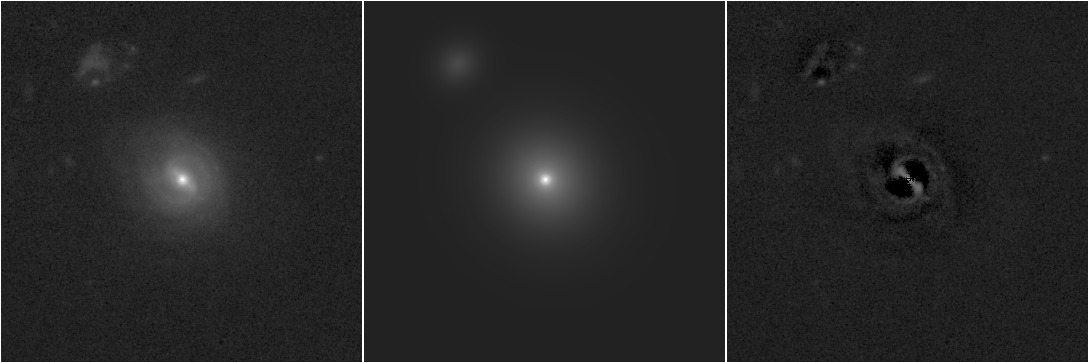
\includegraphics[width=0.8\textwidth]{Together}
\caption{{\tt GALFIT} output for i-band imaging of object 50002399 and a companion. Left: Input image cropped to fit box size. Middle: best fit model containing disk, bulge and PSF components. Right: residuals obtained from subtracting the latter from the former. Even though forcing an axisymmetric model to non-axisymmetric bars leads to strong undersubtraction of the bar features and oversubtraction of the surrounding area, the residuals indicate these contributions are well balanced. Most importantly, the residuals demonstrate the outer regions of the disk are well subtracted, resulting in the most accurate disk profile over the entire region.}\label{examplefigure}
\end{figure*}
%\vspace{8em}
\begin{table*}
\fontsize{9.2}{13}\selectfont
\centering
\begin{tabular*}{.8\textwidth}{@{\extracolsep{\fill}}lccccccc}
\toprule\toprule
 \multicolumn{1}{c}{} &
  \multicolumn{1}{c}{$x$} &
  \multicolumn{1}{c}{$y$} &
  \multicolumn{1}{c}{$m$} &
  \multicolumn{1}{c}{$r_{e}$} &
  \multicolumn{1}{c}{$n$} &
  \multicolumn{1}{c}{$b/a$} &
  \multicolumn{1}{c}{P.A.} \\
  \multicolumn{1}{c}{} &
  \multicolumn{1}{c}{(pix)} &
  \multicolumn{1}{c}{(pix)} &
  \multicolumn{1}{c}{} &
  \multicolumn{1}{c}{(pix)} &
  \multicolumn{1}{c}{} &
  \multicolumn{1}{c}{} &
  \multicolumn{1}{c}{(degrees)}\\
\midrule
  Disk & 501.79 & 502.02 & 19.24 & 32.09 & 1.14 & [0.92] & 43.28\\
  Bulge & [501.00] & [501.83] & 21.56 & 5.08 & 0.37 & [0.92] & [45.26]\\
  Companion & 413.73 & 617.55 & 22.28 & 17.01 & 0.82 & 0.90 & -50.07\\
  PSF & 501.01 & 501.88 & 20.69 &  & & & \\ 
%\vspace{-0.5em} \\
\bottomrule\end{tabular*}\\
 \begin{flushleft}
\vspace{-0.7em}
\hspace{0.1\textwidth}Sky: 6.59e-04 \hspace{5em} $\chi^{2}$: 396480 \hspace{5em} $N_{dof}$: 130301 \\
\vspace{-1em}
\end{flushleft}
\caption{Output {\tt GALFIT} parameters for the best fit of object 50002399. At the redshift of this source each pixel corresponds to 0.22 kpc, so the effective radii are  $r_{e}\sim 7$ kpc and $r_{e} \sim 1$ kpc for the disk and bulge respectively. Parameter values enclosed in square brackets have been held fixed. The disk axis ratio ($b/a$) was held fixed, and bulge $x$ and $y$, $b/a$ and position angle (P.A.) were fixed to similar values as the disk, in order to prevent {\tt GALFIT} from modifying these components to reproduce the non-axisymmetric bar component.}\label{exampletable}
\end{table*}

%at the redshift of this source the physical scale is 0.22 kpc/pixel (pixels are 0.05"), so the disk r_e is ~7 kpc and the bulge r_e is ~1
%The first was resolved by initially setting the sky to zero, which allowed {\tt GALFIT} to let the sky converge to its actual small value. CHECK WHAT HAPPENED WITH THE OTHER FILES (ONLY DISKS?). After the crashes were repaired, I manually improved upon each of the fits before trying to add a bulge. In hindsight I should have proceded to add a bulge sooner,  as much time was wasted attempting to solve problems that could easily have been solved by a bulge addition
\paragraph{} 
During fitting, in addition to the $\chi^{2}$ parameter, I adopted the following characteristics as indicative of a good fit:
\begin{itemize}
\item{\emph{Constant residuals:} even residuals, where neither oversubtraction nor undersubtraction occurs, indicate a good fit. The maximum extend to which this is possible ,however, depends on the smoothness of the light distribution in each galaxy image.}
\item{\emph{Sensible parameters}: parameters were required to be in good accordance with expectations from visually inspecting input images. For example, most galaxies are known to have S\'{e}rsic indices of between 0.1 and 8 \cite{caon93}. Therefore, when the S\`{e}rsic index converged to a value outside this range, $n$ was fixed to a sensible value. In cases where parameters were fixed, care was taken to ensure the fit recovered the maximum bulge luminosity in order to obtain a secure upper limit on bulge flux. }
\item{\emph{Match between bulge and disk}: as bulges are mostly axisymmetric around the same axis as the disk they live in, they should undergo very similar projection and orientation effects. The axis ratio parameter, for instance, is mainly a result of projection (a disk will appear oval due to the inclination of its central axis). Consequently bulge and disk axis ratios and position angles, as well as positions, are expected to be similar, and were constrained to be if not.}
\end{itemize}

\subsubsection{Individual fitting challenges}\label{problems}
Following the above procedures would generate optimal fits in the case of smooth and featureless galaxies in images without artifacts. However, the sample considered in this project was specifically selected to contain disk-dominated galaxies, which often have detailed or asymmetric features that require careful treatment. This section summarises the main issues that arose during fitting, and how they were handled. 
%\begin{itemize}
\paragraph{} Firstly, an important common issue involved companion galaxies with light profiles intersecting those of the main galaxy. In cases where these companions were of considerable size  I fit them simultaneously with the main galaxy, in order to ensure that the extended wings of the companion's light profile were not confused with the main galaxy. 
\paragraph{} Secondly, many galaxies contained irregular features. Spiral arms for instance, could lead to chaotic residuals with both over- and under-subtracted regions. However, this in itself need not generate poor disk luminosities. {\tt GALFIT} generally handles brightness contrast well as part of the optimisation procedure, as long as the image does not contain extremely bright or dark features. To this end, exceptionally bright parts such as starburst regions were masked out. Bars, on the other hand, could lead to incorrect fits, as {\tt GALFIT} would attempt to reconstruct them by rotating and  narrowing the sersic profiles of disks or bulges in order to create a narrow central region. In order to avoid this, I often constrained the axis ratios and position angles of bulge and disk to be similar.
\paragraph{} Thirdly, in some cases dust led to apparent disk asymmetry and obscuration, as exemplified by object 50013002. {\tt GALFIT} does not currently model any components with negative or absorbed luminosity, so optimisation of images containing prominent dust lanes will always lead to erroneously low luminosities, or in worse cases, reproduction of dust induced asymmetry or failure to correctly reproduce obscured features. Theoretically, one could apply a bad pixel mask to dust dominated regions, which forces {\tt GALFIT} to ignore the pixels within the masked region. However, in practice it often turned out that this only amplified obscuration issues. Thus dust masks were avoided where possible. Instead, parameter constraints (e.g. equating bulge and disk centres) were employed to combat asymmetries if necessary. 
\paragraph{} Finally, a number of images contained artifacts, or diffraction spikes. These issues were easily avoided by applying a bad pixel mask.  
\paragraph{} 
Despite these caveats I eventually obtained a reasonable best fit for all objects, apart from object 90044623, where dust effects prevented a convergence to reasonable physical values (see Table \ref{resulttable}).

%Visual inspection of object 90046249, for instance, unveils a bottom black region, as this object is at the very edge of the observation field. The blue dot slightly above it is an artifact from equipment errors.  Both were masked out using a bad pixel mask. Object 90040478 contained a diffraction spike (invisible on the colour image) from a nearby bright star.
%\paragraph{} Finally, several images included companion galaxies. In cases where these companions were of considerable size they were fit simultaneously with the main galaxy, in order to ensure that the extended wings of the companion's light profile were not confused with the main galaxy. 
%Generally galfit handles this well as part of the optimisation so long as there are no extremely bright or dark features on the image.

%talk about bar problems
%A representative example of problems and the general solution is presented in section xxx. 
%Example sheds light on methodology. 

%Companions were subtracted in order to ensure the main galaxy is properly fit. 

%\end{itemize}

%\subsection{Examples}

%In order to clarify the fitting methodology object 50002399 is presented as an example which illustrates general problems and their solution methods. Explain some stuffs. See figure 1, table 1.  

% illustrates the fitting process, and exemplifies

%A bash script was written to automatically create input files with initial value guesses taken from a catalog provided by my supervisor. These input files only contained a disk and a PSF, and initially the luminosity was taken to be equally spread over the PSF and disk. An initial value of $n=2$ was assumed. On the first few runs there were crashes for some of the galaxies, but these crashes could usually be resolved in a fairly straightforward manner, for instance by readjusting initial guesses for the sky values, or removing a troublesome psf on the first try (and adding it back in after having fixed the disk). I then attempted to perfect these PSF + Disk fits before adding a bulge. In hindsight I should have added bulges earlier, as I unnecesarily spent time in the disk-fitting stage fixing issues (high S\'{e}rsic index/poor central residuals) that could easily have been resolved by adding a small bulge. 

%Characteristics of a good fit: 


%\subsection{Initial automated fitting}
%A bash script was written to automatically create input files with initial value guesses taken from a catalog provided by my supervisor. Initially it was assumed that the luminosity was equally spread over the PSF and disk. An initial value of $n=2$ was assumed. On the first few runs there were crashes for some of the galaxies, but these crashes could usually be resolved in a fairly straightforward manner, for instance by readjusting initial guesses for the sky values, or removing a troublesome psf on the first try (and adding it back in after having fixed the disk). 

%\subsection{Optimising the disk and PSF fitting}
%After running this automated series of fits, I tried to manually adjust the fits to improve. This mainly involved the following three processes: 

%\begin{itemize}
%\item{Fitting companions}
%\item{Masking artefacts}
%\item{Masking bright bits of bars, spirals and generally overly bright points}
%\end{itemize}

%\subsection{Adding bulges}



\section{\normalsize RESULTS}\label{results}
\begin{table*}[!t]
 %\centering
\fontsize{9.2}{13}\selectfont

 %\hspace{40em} $\log{M} $($M_{\odot}$)

\begin{tabular}{@{}rrrrrrrccrr@{}}
\toprule\toprule
\multicolumn{1}{c}{} &
  \multicolumn{1}{c}{} &
  \multicolumn{4}{c}{{\tt {\tt GALFIT}} parameters ($I$-band) } &
  %\multicolumn{1}{c}{(pix)} &
  %\multicolumn{1}{c}{} &
  %\multicolumn{1}{c}{} &
  %\multicolumn{1}{c}{(pix)} &
  %\multicolumn{1}{c}{} &
  \multicolumn{1}{c}{} &
  \multicolumn{2}{c}{Significance} &
  %\multicolumn{1}{c}{$L_{BH}$} &
  %\multicolumn{1}{c}{$M_{BH}$} &
  %\multicolumn{1}{c}{} &
  \multicolumn{2}{c}{$\log{M} (M_{\odot}$)} \\ 
  %\multicolumn{1}{c}{($M_{\odot}$)} & 
  %\multicolumn{1}{c}{} \\

\cmidrule(r){3-6} \cmidrule(r){8-9} \cmidrule(r){10-11}

  \multicolumn{1}{c}{OBJNO} &
  \multicolumn{1}{c}{$z$} &
  \multicolumn{1}{c}{$m_{disk}$} &
 % \multicolumn{1}{c}{$r_{e,disk}$} &
  \multicolumn{1}{c}{$n_{disk}$} &
  \multicolumn{1}{c}{$m_{blg}$} &
 % \multicolumn{1}{c}{$r_{e,blg}$} &
  \multicolumn{1}{c}{$n_{blg}$} &
  \multicolumn{1}{c}{$\frac{L_{blg}}{L_{host}}$} &
  \multicolumn{1}{c}{$\sigma_{PS}$} &
  \multicolumn{1}{c}{$\sigma_{blg}$} &
 % \multicolumn{1}{c}{$L_{BH}$} &
 % \multicolumn{1}{c}{$M_{BH}$} &
   \multicolumn{1}{c}{$M_{BH}$} &
  \multicolumn{1}{c}{$M_{host}$} \\
 \midrule
%\linespread{1.3em}
%\rule{0pt}{1.2em}  
\color{red} $50006849$ & \color{red} $0.137$ & \color{red} $17.84^{+0.18}_{-0.18}$ & \color{red} $1.35^{+0.29}_{-0.29}$ & \color{red} $20.46^{+0.07}_{-0.07}$ & \color{red} $2.66^{+0.20}_{-0.20}$ & \color{red} $0.082$ & \color{red} $6$ & \color{red} $6$ & \color{red} $3.3$ & \color{red} $9.6$\\

$90040788$ & $0.204$ & $19.33^{+0.27}_{-0.27}$ & $0.66^{+0.29}_{-0.29}$ & $22.48^{+0.07}_{-0.07}$ & $1.15^{+0.20}_{-0.20}$ & $0.052$ & $6$ & $6$ & $3.8$ & $9.2$\\

$90044879$ & $0.2363$ & $21.92^{+0.23}_{-0.23}$ & $0.59^{+0.33}_{-0.33}$ & $22.20^{+0.16}_{-0.16}$ & $0.35^{+0.27}_{-0.27}$ & $0.436$ & $6$ & $6$ & $3.5$ & $9.1$\\

$50002399$ & $0.3059$ & $19.30^{+0.33}_{-0.33}$ & $1.14^{+0.29}_{-0.29}$ & $21.62^{+0.31}_{-0.31}$ & $0.37^{+0.25}_{-0.25}$ & $0.106$ & $6$ & $6$ & $6.3$ & $9.7$\\

$90042212$ & $0.31$ & $18.98^{+0.31}_{-0.31}$ & $1.85^{+0.25}_{-0.25}$ & $23.30^{+0.07}_{-0.07}$ & $0.23^{+0.20}_{-0.20}$ & $0.018$ & $6$ & $6$ & $4.6$ & $10.1$\\

 $90040805$ & $0.316$ & $20.30^{+0.28}_{-0.28}$ & $1.02^{+0.28}_{-0.28}$ & $23.43^{+0.07}_{-0.07}$ & $0.55^{+0.16}_{-0.16}$ & $0.053$ & $6$ & $6$ & $4.2$ & $9.2$\\

$90040478$ & $0.338$ & $19.29^{+0.28}_{-0.28}$ & $0.54^{+0.28}_{-0.28}$ & $21.69^{+0.09}_{-0.09}$ & $0.94^{+0.22}_{-0.22}$ & $0.099$ & $6$ & $6$ & $4.1$ & $9.8$\\

$50015036$ & $0.375$ & $19.09^{+0.29}_{-0.29}$ & $0.64^{+0.27}_{-0.27}$ & $21.47^{+0.12}_{-0.12}$ & $0.35^{+0.24}_{-0.24}$ & $0.100$ & $6$ & $6$ & $4.4$ & $9.5$\\

$50012252$ & $0.3766$ & $20.62^{+0.29}_{-0.29}$ & $1.24^{+0.27}_{-0.27}$ & $22.70^{+0.14}_{-0.14}$ & $0.41^{+0.26}_{-0.26}$ & $0.128$ & $6$ & $6$ & $4.9$ & $9.0$\\

$50003033$ & $0.411$ & $20.63^{+0.28}_{-0.28}$ & $0.30^{+0.28}_{-0.28}$ & $22.32^{+0.14}_{-0.14}$ & $0.87^{+0.26}_{-0.26}$ & $0.174$ & $6$ & $6$ & $4.4$ & $9.4$\\

 $50010422$ & $0.4725$ & $21.09^{+0.33}_{-0.33}$ & $0.61^{+0.25}_{-0.25}$ & $21.95^{+0.27}_{-0.27}$ & $0.35^{+0.29}_{-0.29}$ & $0.312$ & $6$ & $6$ & $4.3$ & $9.3$\\

$50009140$ & $0.4745$ & $22.12^{+0.21}_{-0.21}$ & $0.29^{+0.31}_{-0.31}$ & $22.74^{+0.12}_{-0.12}$ & $1.00^{+0.24}_{-0.24}$ & $0.361$ & $6$ & $6$ & $4.2$ & $8.7$\\

$50011136$ & $0.5124$ & $20.07^{+0.33}_{-0.33}$ & $0.60^{+0.29}_{-0.29}$ & $22.30^{+0.31}_{-0.31}$ & $0.12 ^{+0.25}_{-0.25}$ & $0.114$ & $6$ & $6$ & $6.7$ & $9.5$\\

\color{red} $90044623$ & \color{red} $0.576$ & \color{red} $22.64^{+0.07}_{-0.07}$ & \color{red} $0.38^{+0.20}_{-0.20}$ & \color{red} $21.93^{+0.06}_{-0.06}$ & \color{red} $9.84^{+0.09}_{-0.09}$  & \color{red} $0.658$ & \color{red} $6$ & \color{red} $6$ & \color{red} $4.6$ &\color{red}$9.0$\\

$50007764$ & $0.5951$ & $21.28^{+0.24}_{-0.24}$ & $1.13^{+0.32}_{-0.32}$ & $23.10^{+0.07}_{-0.07}$ & $0.86^{+0.20}_{-0.20}$ & $0.158$ & $6$ & $6$ & $5.0$ & $9.0$\\

$90107689$ & $0.622$ & $21.14^{+0.29}_{-0.29}$ & $0.57^{+0.37}_{-0.37}$ & $26.73^{+0.21}_{-0.21}$ & $0.10^{+0.31}_{-0.31}$ & $0.006$ & $6$ & $4$ & $4.9$ & $9.0$\\

 $10001051$ & $0.634$ & $22.97^{+0.24}_{-0.24}$  & $0.69^{+0.32}_{-0.32}$ & $24.24^{+0.12}_{-0.12}$ & $0.49^{+0.24}_{-0.24}$ & $0.237$ & $5$ & $6$ & $5.6$ & $9.4$\\

$50012060$ & $0.6378$ & $20.73^{+0.28}_{-0.28}$ & $0.68^{+0.28}_{-0.28}$ & $23.45^{+0.07}_{-0.07}$ & $0.97^{+0.20}_{-0.20}$ & $0.075$ & $6$ & $6$ & $5.2$ & $9.7$\\

$50013002$ & $0.6379$ & $21.77^{+0.07}_{-0.07}$ & $0.50^{+0.20}_{-0.20}$ & $22.71^{+0.07}_{-0.07}$ & $0.90^{+0.20}_{-0.20}$ & $0.296$ & $4$ & $6$ & $6.0$ & $9.7$\\

$90041480$ & $0.6432$ & $21.49 ^{+0.21}_{-0.21}$ & $0.64^{+0.31}_{-0.31}$ & $24.89^{+0.07}_{-0.07}$ & $0.63^{+0.20}_{-0.20}$ & $0.042$ & $1$ & $6$ & $4.5$ & $9.3$\\

$90045545$ & $0.654$ & $23.3^{+0.14}_{-0.14}$ & $0.30^{+0.26}_{-0.26}$ & $23.08^{+0.07}_{-0.07}$ & $0.50^{+ 0.20}_{-0.20}$ & $0.550$ & $6$ & $6$ & $4.7$ & $9.2$\\

$90043959$ & $0.6741$ & $23.81^{+0.16}_{-0.16}$ & $0.35^{+0.27}_{-0.27}$ & $25.27^{+0.07}_{-0.07}$ & $0.13^{+0.20}_{-0.20}$ & $0.207$ & $0$ & $6$ & $4.5$ & $8.3$\\

$90042183$ & $0.7213$ & $22.25^{+0.35}_{-0.35}$ & $0.95^{+0.27}_{-0.27}$ & $26.13^{+0.16}_{-0.16} $ & $0.14^{+0.27}_{-0.27}$ & $0.027$ & $6$ & $6$ & $5.2$ & $9.8$\\

$90046249$ & $0.734$ & $22.43^{+0.21}_{-0.21}$ & $0.7 ^{+0.31}_{-0.31}$ & $23.87^{+0.05}_{-0.05}$ & $0.88^{+0.18}_{-0.18}$ & $0.210$ & $0$ & $5$ & $6.6$ & $10.0$\\

  $90046086$ & $0.7373$ & $22.05^{+0.28}_{-0.28}$ & $0.71^{+0.28}_{-0.28}$ & $22.86^{+0.21}_{-0.21}$ & $0.78^{+0.31}_{-0.31}$ & $0.322$ & $6$ & $6$ & $5.2$ & $10.4$\\

  $50013273$ & $0.9712$ & $21.62^{+0.32}_{-0.32}$ & $0.58^{+0.24}_{-0.24}$ & $22.68^{+0.24}_{-0.24}$ & $0.11^{+0.32}_{-0.32}$ & $0.274$ & $6$ & $6$ & $5.3$ & $10.2$\\

 % 50006849 & 0.137 & 17.76 & 58.75 & 1.35 & 20.38 & 9.41 & 2.66 &$>$6&$>$6& 0.082 & 9.6\\
  %90040788 & 0.204 & 19.37 & 28.94 & 0.66 & 22.52 & 2.96 & 1.15 &$>$6&$>$6& 0.052 & 9.3\\
  %90044879 & 0.2363 & 21.98 & 25.47 & 0.59 & 22.26 & 12.86 & 0.35 &$>$6&$>$6& 0.436 & 9.1\\
  %50002399 & 0.3059 & 19.24 & 32.09 & 1.14 & 21.56 & 5.08 & 0.37 &$>$6&$>$6& 0.106 & 10.2\\
  %90042212 & 0.31 & 18.9 & 60.51 & 1.85 & 23.22 & 2.72 & 0.23 &$>$6&$>$6& 0.018 & 10.3\\
  %90040805 & 0.316 & 20.32 & 24.91 & 1.02 & 23.45 & 7.8 & 0.55 &$>$6&$>$6& 0.053 & 9.6\\
 % 90040478 & 0.338 & 19.36 & 67.69 & 0.54 & 21.76 & 12.83 & 0.94 &$>$6&$>$6& 0.099 & 10.2\\
  %50015036 & 0.375 & 19.11 & 48.62 & 0.64 & 21.49 & 9.47 & 0.35 &$>$6&$>$6& 0.1 & 10.2\\
  %50012252 & 0.3766 & 20.56 & 29.69 & 1.24 & 22.64 & 5.56 & 0.41 &$>$6&$>$6& 0.128 & 9.6\\
  %50003033 & 0.411 & 20.68 & 34.75 & 0.3 & 22.37 & 6.13 & 0.87 &$>$6&$>$6& 0.174 & 10.0\\
 % 50010422 & 0.4725 & 21.19 & 16.51 & 0.61 & 22.05 & 3.22 & 0.35 &$>$6&$>$6& 0.312 & 10.2\\
  %50009140 & 0.4745 & 22.21 & 34.55 & 0.29 & 22.83 & 20.81 & 1.0 &$>$6&$>$6& 0.361 & 9.6\\
  %50011136 & 0.5124 & 20.12 & 34.88 & 0.6 & 22.35 & 5.91 & 0.12 &$>$6&$>$6& 0.114 & 10.5\\
 % \color{red} 90044623 & \color{red} 0.576 & \color{red} 21.73 & \color{red} 37.14 & \color{red} 0.38 & \color{red} 21.02 & \color{red} 2299 & \color{red} 9.84 & \color{red} $>$6& \color{red} $>$6& \color{red} 0.658 & \color{red} 11.9\\
%90044623 & 0.576 & 21.73 & 37.14 & 0.38 & 21.02 & 2299.37 & 9.84 &$>$6&$>$6& 0.658 & 11.9\\ 
  %50007764 & 0.5951 & 21.18 & 34.52 & 1.13 & 23.0 & 3.6 & 0.86 &$>$6&$>$6& 0.158 & 10.1\\
  %90107689 & 0.622 & 21.18 & 24.98 & 0.57 & 26.77 & 3.42 & 0.1 &$>$6& 4 & 0.006 & 10.1\\
  %50001051 & 0.634 & 23.01 & 20.52 & 0.69 & 24.28 & 7.26 & 0.49 & 5 &$>$6& 0.237 & 10.4\\
  %50012060 & 0.6378 & 20.81 & 22.12 & 0.68 & 23.53 & 1.89 & 0.97 &$>$6&$>$6& 0.075 & 9.3\\
  %50013002 & 0.6379 & 22.19 & 75.12 & 0.5 & 23.13 & 15.39 & 0.9 & 4 &$>$6& 0.296 & 10.4\\
  %90041480 & 0.6432 & 21.51 & 48.02 & 0.64 & 24.91 & 4.84 & 0.63 & 1 &$>$6& 0.042 & 10.3\\
  %90045545 & 0.654 & 23.38 & 44.67 & 0.3 & 23.16 & 21.24 & 0.5 &$>$6&$>$6& 0.55 & 10.0\\
  %90043959 & 0.6741 & 23.93 & 24.49 & 0.35 & 25.39 & 11.24 & 0.13 & 0 &$>$6& 0.207 & 9.2\\
  %90042183 & 0.7213 & 22.26 & 15.3 & 0.95 & 26.14 & 2.3 & 0.14 &$>$6&$>$6& 0.027 & 10.7\\
  %90046249 & 0.734 & 22.41 & 30.0 & 0.7 & 23.85 & 7.7 & 0.88 & 0 & 5 & 0.21 & 10.7\\
  %90046086 & 0.7373 & 22.07 & 21.54 & 0.71 & 22.88 & 3.57 & 0.78 &$>$6&$>$6& 0.322 & 11.2\\
  %50013273 & 0.9712 & 21.69 & 28.78 & 0.58 & 22.75 & 4.44 & 0.11 &$>$6&$>$6& 0.274 & 11.0\\
\bottomrule
\end{tabular}
\caption{Properties of the sample of 26 bulgeless candidates sorted by ascending redshift. Values for $m_{disk}$, $r_{e,disk}$, $n_{disk}$, $m_{blg}$, $r_{e,blg}$ and $n_{disk}$ were obtained with {\tt GALFIT} from $I$-band imaging. Conservative errors on these values have been obtained from Simmons \& Urry 2008 \cite{2008ApJ...683..644S}.  Fit parameters demonstrate that object 90044623 could not be fit correctly and that object 50006849 contains a classical bulge. Both are indicated in red and were removed from the sample. 13 galaxies have sizeable pseudobulges of $L_{blg}/L_{tot} > 0.15$, with the other 11 galaxies being predominantly bulgeless. $\sigma_{psf}$ and $\sigma_{blg}$ quantify the significance of adding a psf or bulge respectively. Black hole masses are lower limits based on Eddington limit accretion. Disk masses have been calculated following Bell \& De Jong 2001 \cite{2001ApJ...550..212B}}\label{resulttable}
\end{table*}
\subsection{ {\tt GALFIT} results}
Best fit parameters for all 26 candidate objects are presented in Table \ref{resulttable}. I renormalised magnitudes to the well measured values from GOODS\cite{2012ApJS..200....9G}, and obtained errors on the {\tt GALFIT} parameters following Simmons \& Urry 2008 \cite{2008ApJ...683..644S}. Because these errors are derived from automated batch fitting, they form very conservative upper limits. My sample has been carefully individually fit,  and actual errors are likely to be much smaller. 
\paragraph{} The $n_{blg}$ value for object 50006849 indicates a classical bulge, so this object was removed from the mergerless sample. Object 90044623 was rejected for having unphysical fit parameters. 13 galaxies contain a significant pseudo-bulge contribution $L_{blg}/L_{host} > 0.15$, the other 11 are predominantly bulgeless. 
\paragraph{} I computed disk masses following Bell \& de Jong \cite{2001ApJ...550..212B} with K-corrections from Poggianti \cite{1997AAS..122..399P} , the details of which are provided in Appendix \ref{diskmass}. 
%Section \ref{bhmass} discusses black hole mass calculations. 
\paragraph{} $\sigma_{PS}$ and $\sigma_{blg}$ quantify the statistical significance of adding a point source or bulge component to the model respectively. These values have been obtained from an F-test and indicate the amount of standard deviations by which the more sophisticated model improves on the simpler one. Details of this procedure are provided in Appendix \ref{ftest}.


\paragraph{} It is interesting to note that the best fit parameters in Table \ref{resulttable} differ significantly from the values obtained  for a single S\'{e}rsic profile in the ACS-GC \cite{2012ApJS..200....9G}. The vast majority of ACS-GC fits have significantly higher $n$ values, on average $\sim 1.3$ higher. The difference is most extreme in the case of object 50002399, where the AGN-GC value is 6.32 too high.  These results are expected, since in a single disk model, {\tt GALFIT} will attempt to reconstruct a point source by centralising the light profile, thus increasing $n$. Additionally, in Section \ref{autofitting} I noted how several fits improved significantly from the addition of bulges. Together these results demonstrate the importance of sophisticated models in automated fitting procedures, indicating the need to model both disk, bulge and PSF in order to properly extract galaxy morphologies in the case of active galaxies. 

\subsection{\normalsize  Black hole masses}\label{bhmass}
The Eddington limit is the maximum bolometric luminosity an accreting BH can achieve when radiation pressure emmited from accreting matter is in hydrostatic equilibrium with the graviational pull exerted by the black hole. At the Eddington limit, there is a relation between mass and luminosity \cite{2013heai.book.....C}: 
\begin{equation}
L_{edd} = 1.3 \cdot 10^{38} \left( \frac{M_{edd}}{M_{\odot}} \right) \mathrm{ \frac{erg}{sec}}
\label{eddington}
\end{equation}
If the bolometric luminosity is assumed to be the Eddington luminosity, Equation \ref{eddington} gives a lower bound on the black hole mass. This can be seen by considering the fact that if the observed luminosity is below the Eddington limit, it is lower than the maximum value that can still be contained by gravity. If the observed luminosity stays the same, this implies that the gravitational pull of the black hole must be stronger for the black hole to be able to gravitationally counteract the radiation pressure, implying a higher black hole mass.
\paragraph{} I used bolometric luminosities obtained from X-ray hard band luminosities to compute Eddington limit lower bounds on black hole masses. These lower limits are quite conservative, as most black holes accrete well below their Eddington limit. For instance, the AGN in Simmons et al.  2013 with firm black hole masses had a mean of $L \approx 0.065 \: L_ {Edd}$\cite{Simmons01032013} . I used this value to obtain an indication of the more probable real value of the black hole masses. It must be noted, however, that 8 X-ray hard band luminosities were only provided as upper limits. In these cases, it is possible that the Eddington limit masses are not a secure lower limit, as the bolometric luminosities could in fact be lower. In all subsequent figures these objects were marked by an inverted triangle. 
\paragraph{} Black hole mass relations using the results in this section are displayed in Figure \ref{plot1} and Figure \ref{plot2}. 

%The results of this section are summarised in Figure \ref{plot1} shows the relation of $M_{BH}$ with $M_{bulge}$ and $M_{host}$. Figure \ref{plot2} demonstrates how the ratio $\frac{M_{BH}}{M_{bulge}}$ changes with redshift. 



%The lower masses are quite conservative. Discuss Eddington rates. For instance in Simmons et al, the BHs with precise masses from broad emission lines have mean $ L =0.065 L_{edd}$. If this is assumed, BH masses are more in line with expectations from SMBHs. 

%If the real $L_BH$ is lower than the one found here, the eddington lower limit could be lower than the lower limit I found, implying that the actual mass could be lower. 


%It must be  noted that some sources have bla. 
%\subsection{X-ray purity}\label{xray}
%If not all X-ray emission is from AGN, but instead from binaries or starburst our lower limits might be too high (actual AGN luminosity is lower so the lower limit is lower). To study this, consider X-ray emission (if hard X-ray > 43 it is likely to be AGN). Also consider correlation between PSF flux and AGN flux (exclude those PSFs which the F-test shows to be insignificant). Show plot (there is a correlation!). Discuss hardness ratios. Based on these criteria, decide which AGN lower limits are secure (and which might be lower). 


%\section{\normalsize GALAXY-BLACK HOLE MASS RELATIONS}
%Figure \ref{plot1} presents relations between the black hole mass and the disk and bulge mass.  \ref{plot2}

\begin{figure*}[!t]
\centering

\vspace{-1em}

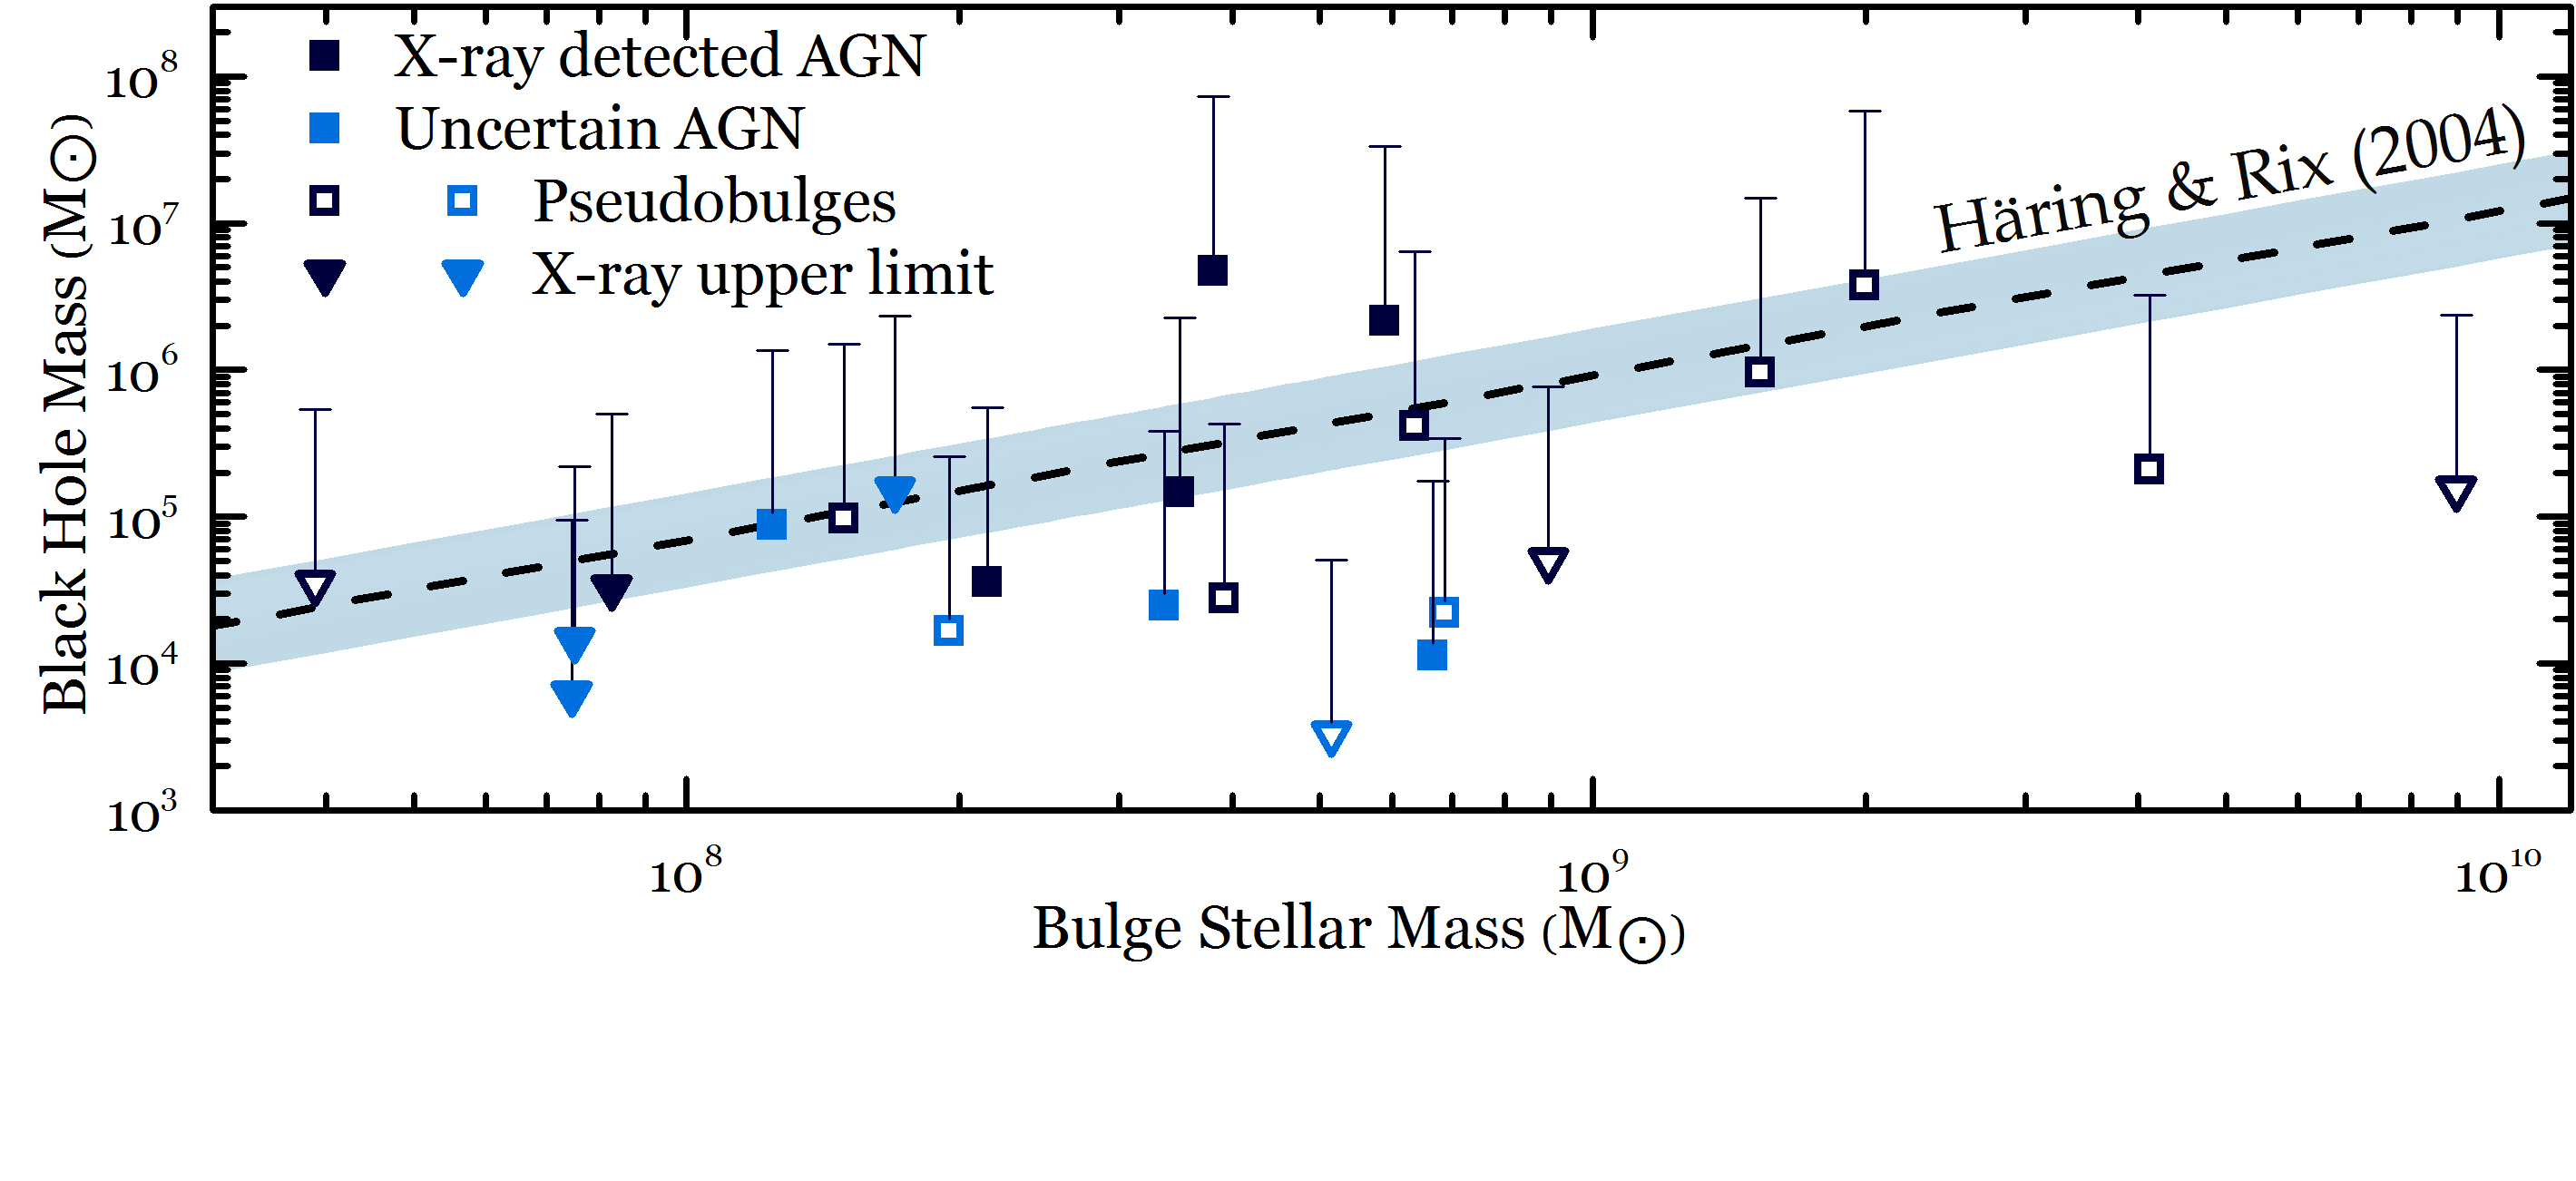
\includegraphics[width=0.9\textwidth]{Graph2}

\vspace{-2.8em}

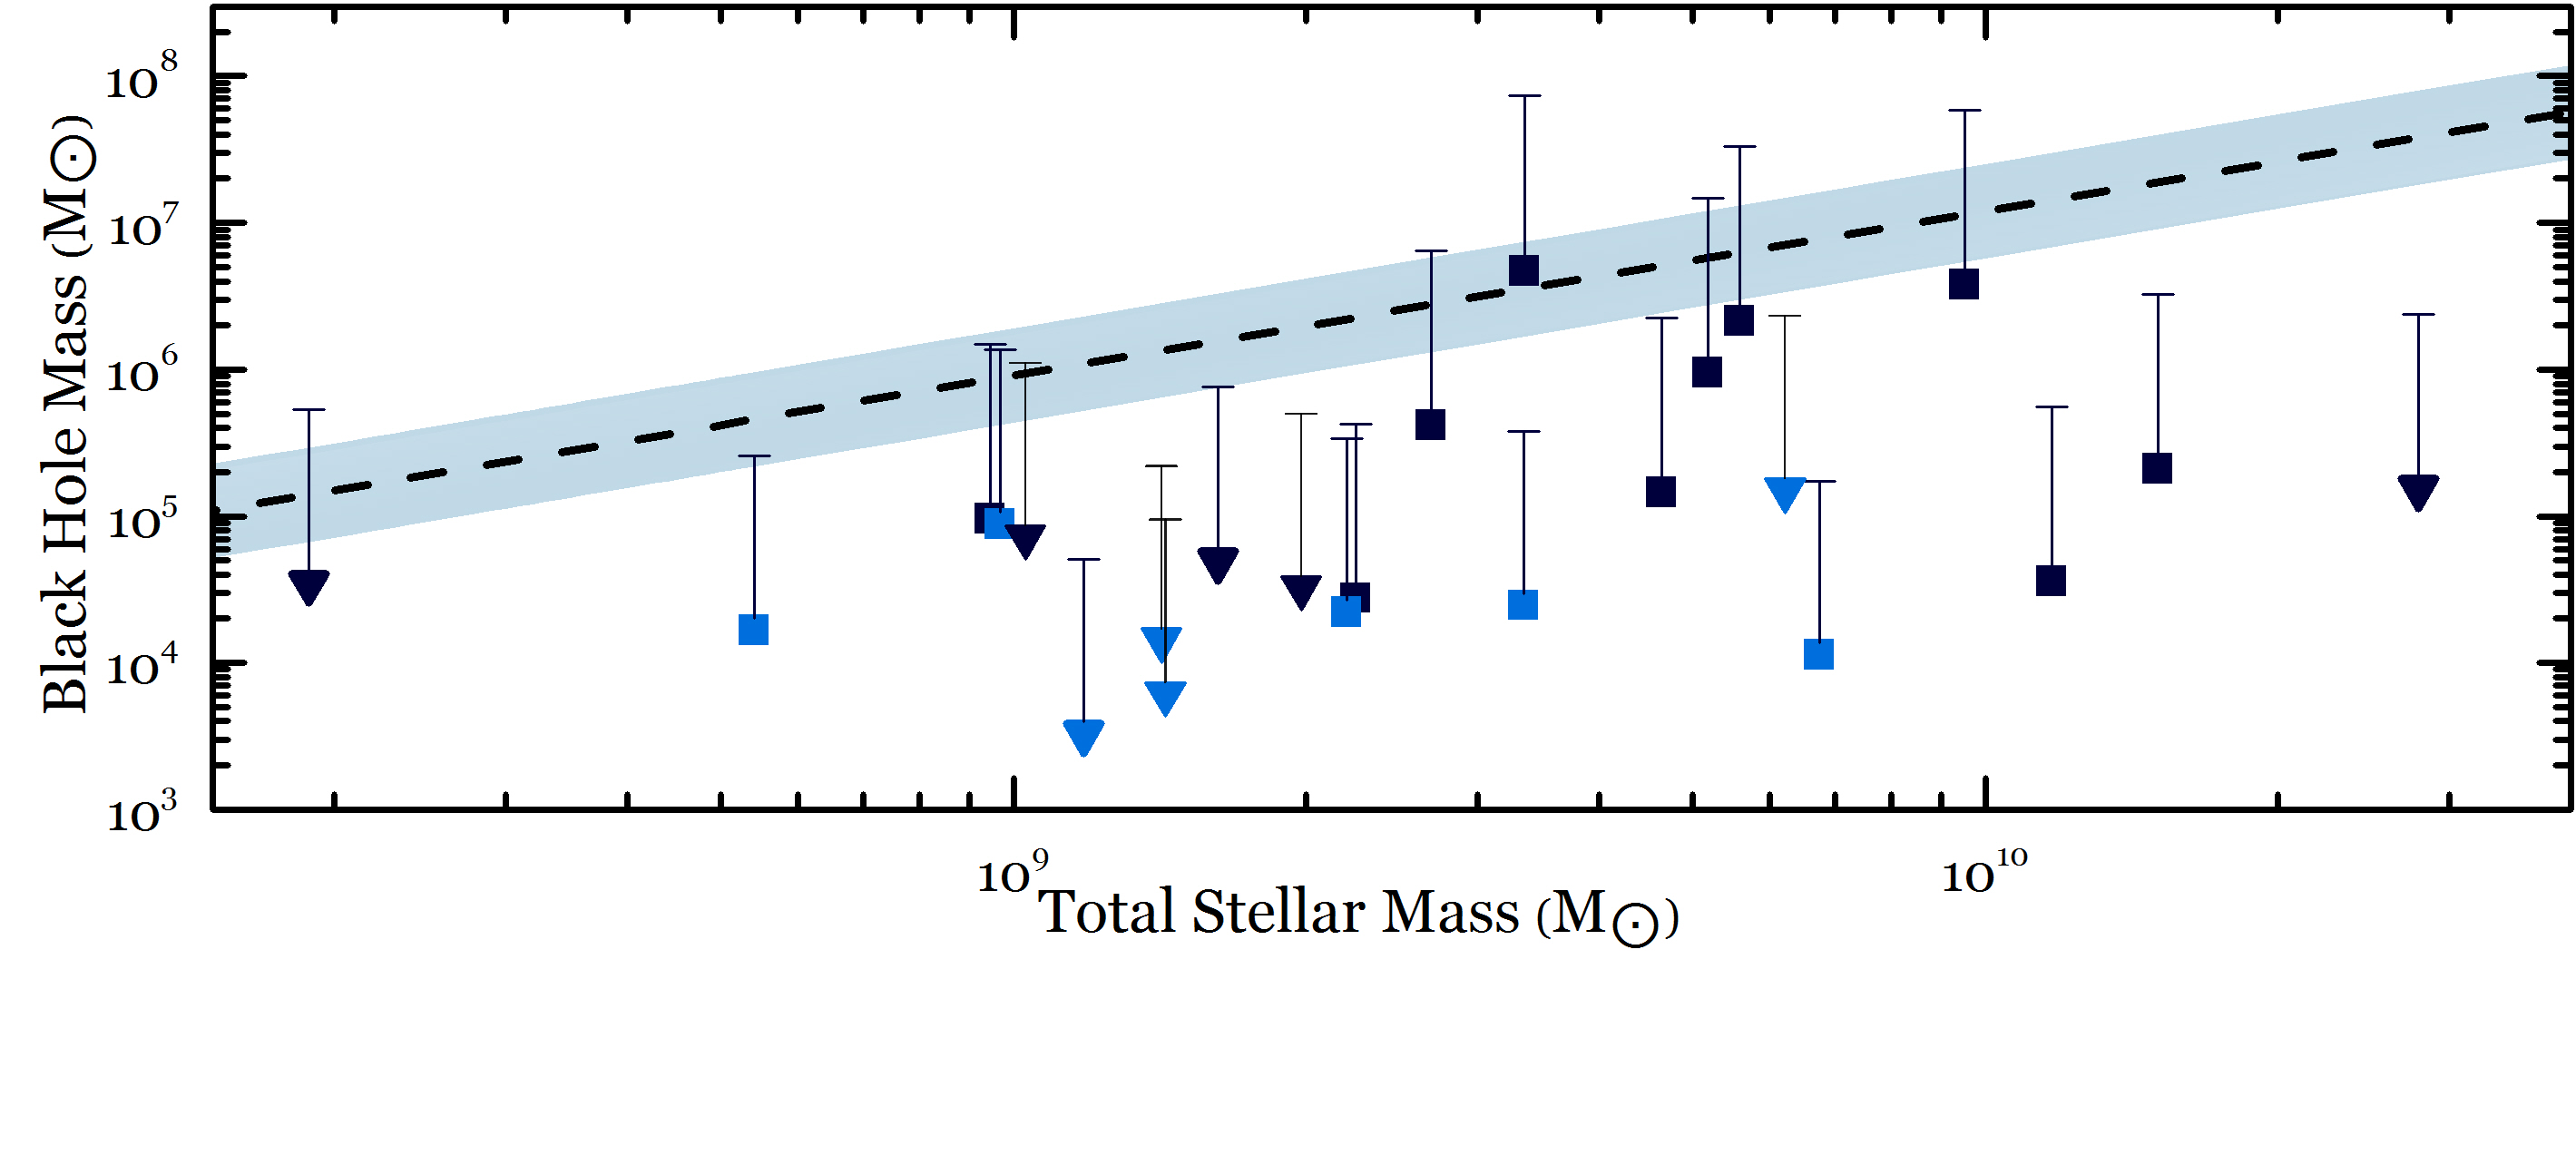
\includegraphics[width=0.9\textwidth]{Graph1_2}
\vspace{-3.5em}
\caption{Black hole mass versus bulge mass (top) and total stellar host galaxy stellar mass (bottom). Black hole masses are lower bounds assuming Eddington limit accretion, caps indicate more likely black hole masses assuming an Eddington ratio of 0.065. The 10 galaxies with sizeable ($L_{bulge}/L_{host} >  0.15$) pseudo-bulges are indicated by open markers, whereas the remaining 15 bulgeless galaxies are indicated by solid markers. Triangular markers show objects for which X-ray luminosities are an upper limit, implying that the $M_{BH}$ lower bounds on these objects could possibly be $lower$.  Light blue data points designate objects for which AGN selection criteria\cite{bla} did not indicate a likely AGN and these could consitute star formation galaxies. Both plots demonstrate a tentative agreement with the relation between bulge/elliptical stellar mass and black hole mass from H\"{a}ring \& Rix 2004 \cite{Haring:2004hr} indicated by the dashed line. Especially if less importance is attached to the uncertain AGN, black hole mass limits are mostly consistent with the H\"{a}ring \& Rix relation within its 0.3 dex scatter, if the relation is assumed to hold for bulge and total stellar mass.  }\label{plot1}
\end{figure*}
%Bulge stellar masses were obtained from the ratio between bulge and total host luminosities as indicated by {\tt {\tt GALFIT}}. 
%None of these objects have detected classical bulges.
%Total stellar masses ($M_{disk} + M_{bulge}$) were computed from mass-to-light ratios using $V-I$ colour following Bell \& de Jong 2001\cite{bla}. 





\section{\normalsize DISCUSSION}\label{discussion}

\begin{figure}[!t]
%\centering
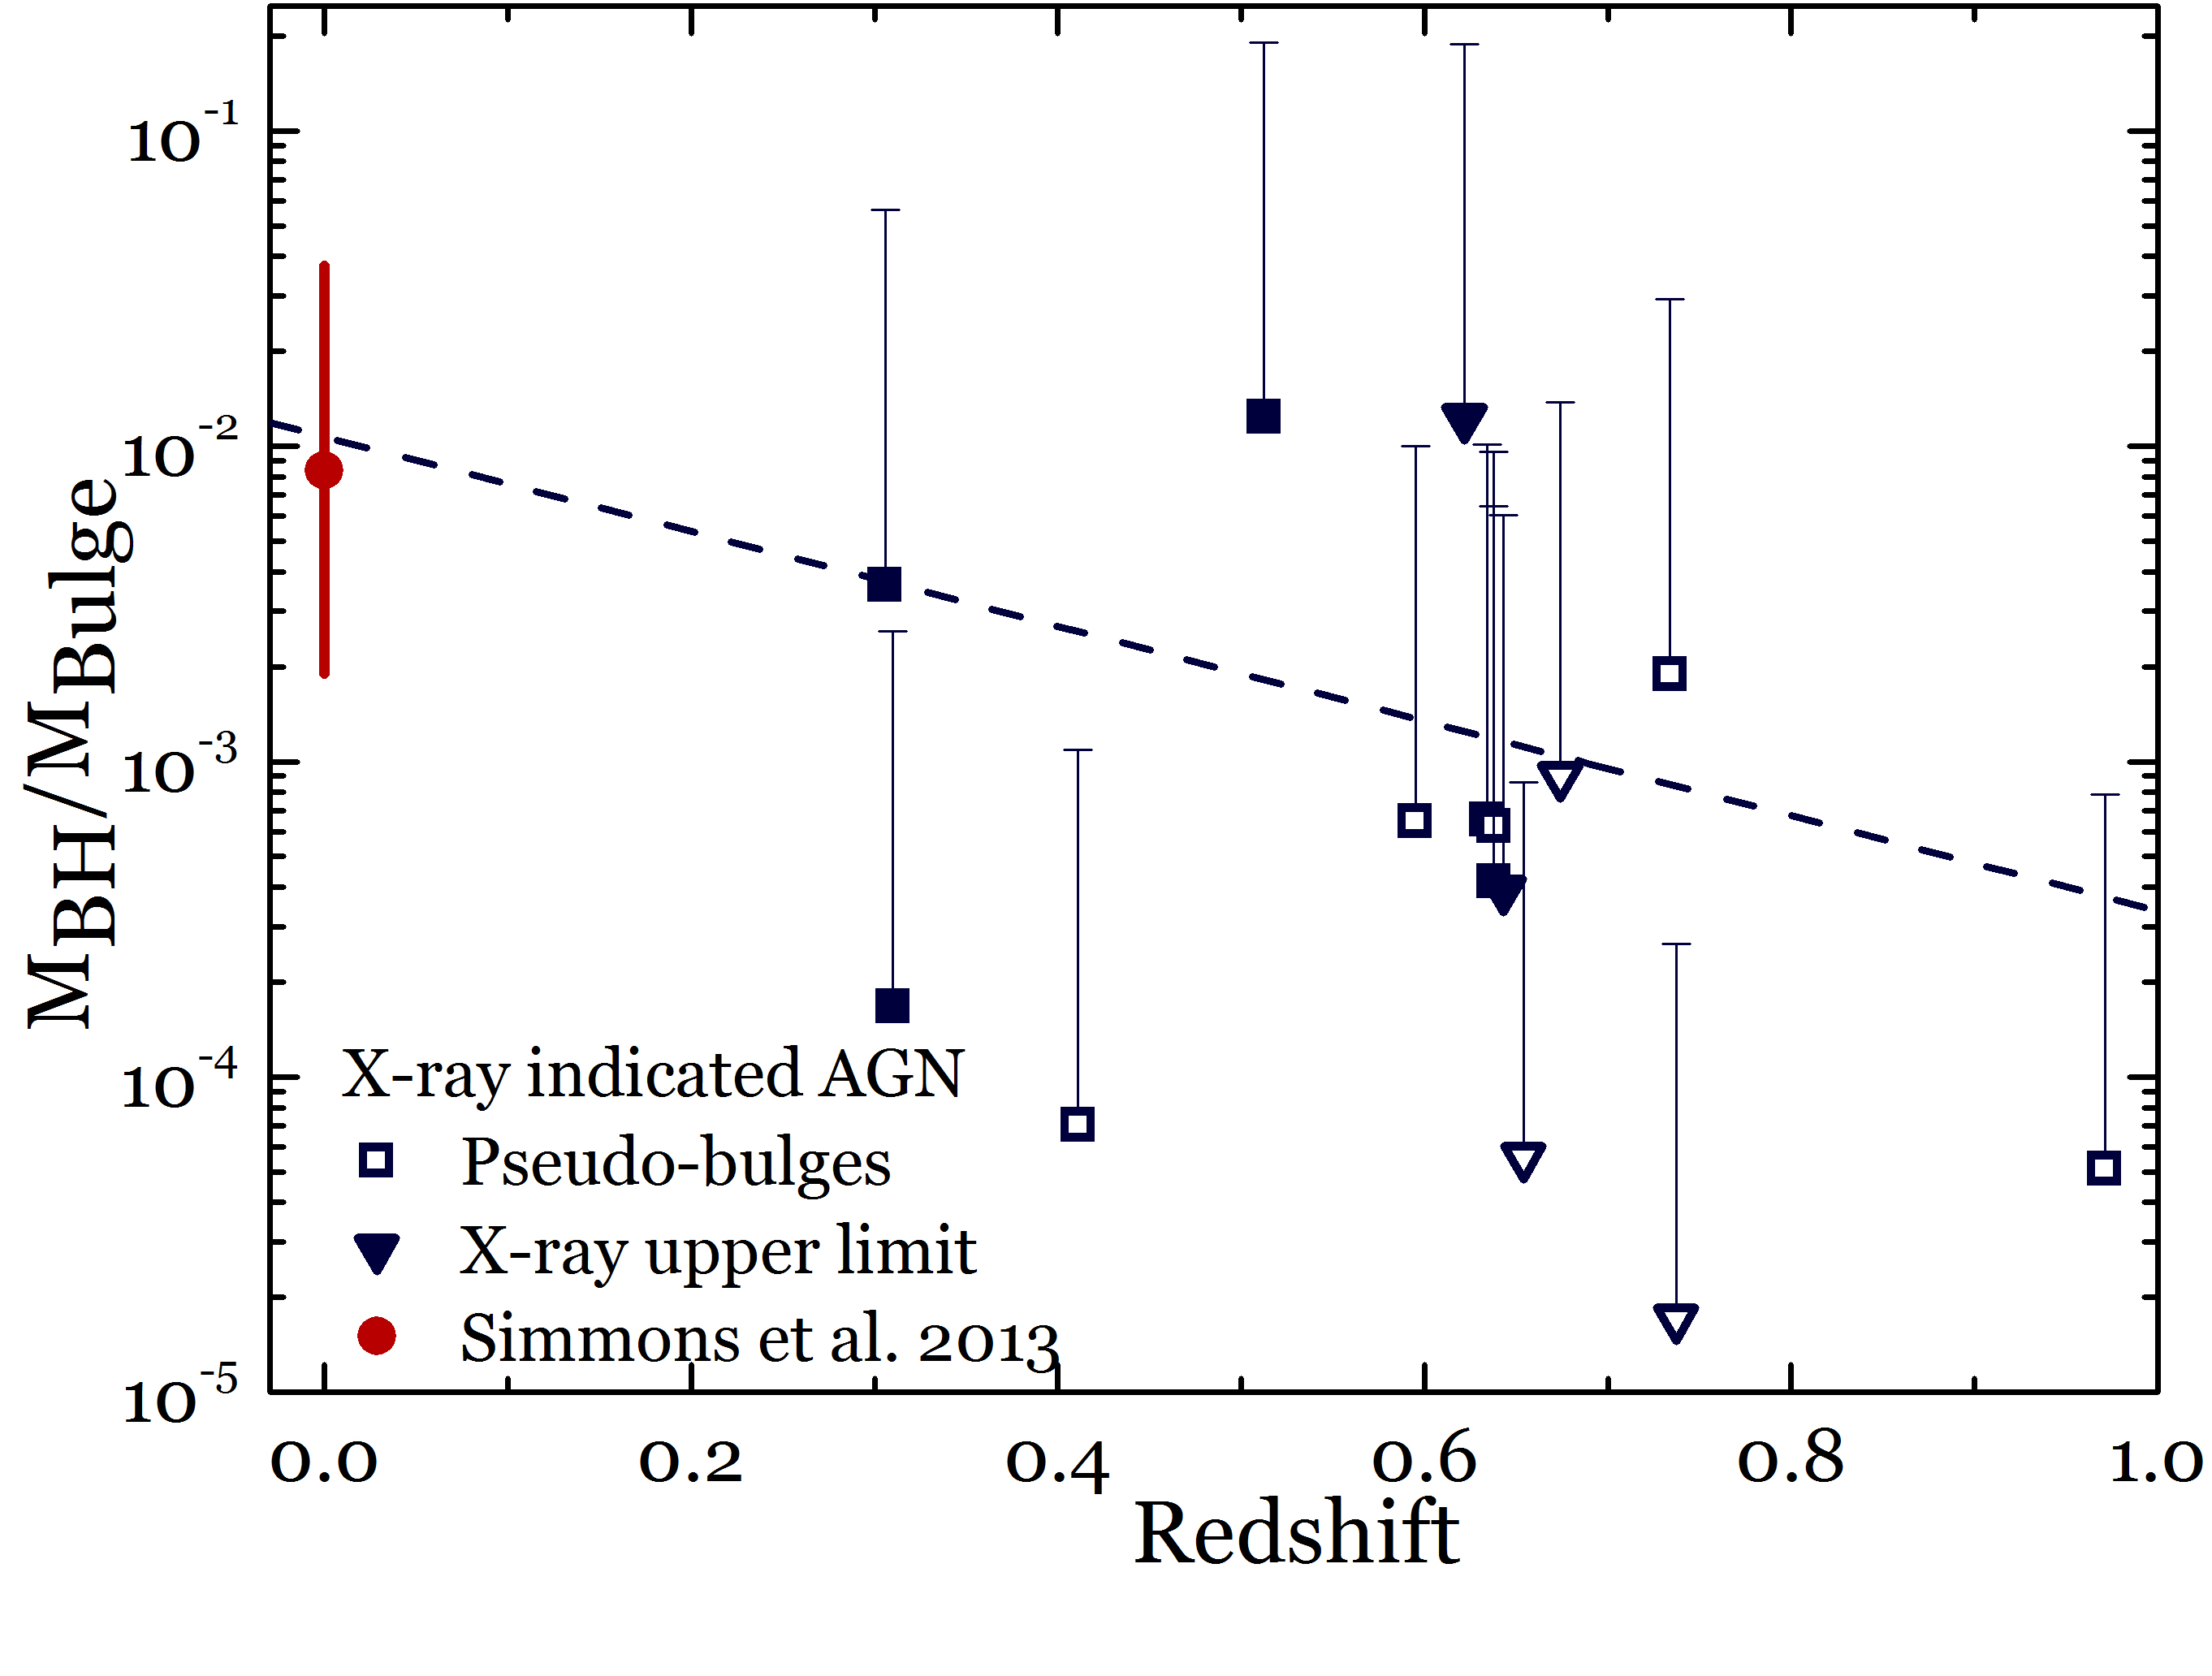
\includegraphics[width=0.99\textwidth]{Graph3}
%\vspace{-2em}
\caption{Ratio of black hole to bulge mass as a function of redshift, for all 15 X-ray detected AGN. Of these, 8 hosts contain sizeable pseudo-bulges ($L_{bulge}/L_{host} >  0.15$), the remaining 7 are predominantly bulgeless. In the case of triangular markers, X-ray luminosities were an upper limit, so for these, the Eddington limit masses could be too high. The dashed line indicates the best fit for these 14 hosts. The average value found in Simmons et al. 2013 for $z\sim 0$  is shown in red and falls neatly onto the relation. Including it does not change the best fit, but halves the errors resulting in a best fit of $\log{( \frac{M_{BH}}{M_{bulge}} )} =  -2.0 (\pm 0.5) - 1.4 (\pm 0.9) z $. These results hint that over time, black holes ``outgrow" their pseudo-bulges.}\label{plot2}
\end{figure}

%At the high redshifts considered in Figure \ref{plot1} ($z_{average} = 0.6$), black holes and bulges obey the H\"{a}ring \& Rix relation, while the local black holes in Simmons et al. are all larger than the relation suggests based on their bulge mass.  


As mentioned in Section \ref{intro}, according to current galaxy formation theories, galaxies are built up hierarchically through a series of mergers, which are also thought to be responsible for the growth of supermassive black holes. In this picture, where the coevolution of hosts and their black holes is driven by mutual growth through mergers, large mergerless galaxies with SMBHs are expected to be rare. Moreover, considering the fact that only a small fraction of SMBHs is in an actively growing phase, mergerless AGN hosts are predicted be even rarer. Nevertheless I have identified 24 such galaxies, of which 11 are predominantly bulgeless (pseudo-bulge contribution of $ < 0.15 \% $ ), and the other 13 contain more sizeable pseudo-bulges. Despite the fact that pseudo-bulges are indicative of a slightly violent history including strong disk instabilities such as bars and clumps, they are still formed in merger-free processes \cite{2012ApJ...756...26M}, implying a merger-free history for all 24 objects. This project thus adds to the local sample of mergerless AGN hosts found in Simmons et al. 2013, strengthening the case for black hole growth independent of mergers. Furthermore, the galaxies in this sample follow the same quantative mass relations as merger-dominated classical bulges and ellipticals (see Figure \ref{plot1}).
\paragraph{} It must be noted that the results presented here have a several limitations in their accuracy. First of all, the k-corrections  were performed under likely unrealistically simple assumptions, and different methods could give a factor of 2 (0.3 dex) offset in disk mass. Furthermore, bulge masses were computed with the aim of maximising any possible bulge contribution, so should be read as a secure upper limit on bulge mass. On top of this, as mentioned in section \ref{bhmass}, X-ray catalogs merely  provided an upper limit on the point source flux for 8 objects. In these cases it is possible that the actual point source luminosity is lower, which would result in a lower Eddington limit, as implied by Equation \ref{eddington}.
\subsection{Black hole-bulge relations}
 Nevertheless, even with these limitations in mind, Figure \ref{plot1} indicates agrement with earlier relations. H\"{a}ring \& Rix \cite{Haring:2004hr} found a local relation between bulge mass and black hole mass applicable to classical bulges, indicated by the dashed line with the 0.3 dex observed scatter in light blue. Within the black hole mass limits, the  relations between $M_{BH}$ and pseudo-bulge $M_{bulge}$ observed in this project agree fairly well with this relation, especially disregarding galaxies indicated in light blue, which do not have X-ray indicated AGN. This conclusion disagrees with local results found in Simmons et al. \cite{Simmons01032013}, where all lower limits on the black hole mass are higher than expected from H\"{a}ring \& Rix. This trend towards higher $M_{BH}/M_{bulge}$ for descending $z$ is also observed throughout the redshift range of the current sample. Figure \ref{plot2} illustrates the relation between $M_{BH}/M_{bulge}$  and redshift. The local average result for Simmons et al. is in good agreement with the best fit from my results. Figure \ref{plot2} tentatively suggests that black holes can accrete mass over time disproportionally to their pseudo-bulges, which would imply calm BH-accretion independently of galaxy mergers, but also of dynamical processes that grow pseudo-bulges. 
\paragraph{} Futhermore, it is interesting to note the average disk mass in Simmons et al. is $M_{BH} =1.51 \times 10^{10} \: \mathrm{M_{\odot}}$ for an average redshift of $z=0.036$. To compare, the average disk mass in my sample is $M_{BH} = 4.74 \times 10^{9} \: \mathrm{M_{\odot}}$ for an average redshift of $z=0.509$. If my sample is hypothesised to be the progenitors of the Simmons et al. sample, this would imply a star formation rate of $~ 1 \: \mathrm{M_{\odot}/year}$, which is a very typical value \cite{2004MNRAS.351.1151B}. Care must be taken regarding the interpretation of this result, as  pseudo-bulge sizes for part of my sample precludes these galaxies from being progenitors of the Simmons et al. galaxies, which barely contain pseudo-bulges at all. My other 11 bulgeless galaxies though, are consistent with having evolved into galaxies like in Simmons et al, a hypothesis which, if true, could explain the redshift trend observed in \ref{plot2}. 

%This trend would suggest that over time, black holes outgrow their host pseudo-bulges. 
\subsection{Black hole-host relations}
If the H\"{a}ring \& Rix relation is extended to include total stellar mass as well as bulge mass, it would describe elliptical galaxies, as elliptical galaxies have similar light profiles (and consequently mass profiles assuming a constant mass-to-light ratio) to large classical bulges. Notably the current sample of mergerless disk galaxies also largely follows this predicted relation for elliptical galaxies, as indicated by Figure \ref{plot1}. Simmons et al. 2013 found a similar agreement. Plots of $M_{BH}/M_{host}$ versus redshift show no significant slope and are consistent with the relation being flat. Such a flat redshift dependence has earlier been observed for merger dominated ellipticals and galaxies with significant classical bulges \cite{2011ApJ...741L..11C}\cite{2011ApJ...734...92J}. The fact that mergerless galaxy follow the same black hole-disk mass relations as expected for merger dominated elliptical galaxies, (and possibly even the same redshift dependence) suggests that mergers may not be the fundamental process driving this galaxy-SMBH coevolution. 

%since the simmons et al galaxies are not massive enough, and also have too many pseudo-bulges, it is nog likely that the current sample would be their progenitors. 

\section{\normalsize CONCLUSION}
Of a candidate sample of 26 bulgeless AGN candidates, parametric morphological fitting indicated that, 11 are predominantly  bulgeless, with bulge contributions of less than 15\%. The other 13 objects have significant pseudo-bulges,  implying that a merger-free history for all 24 galaxies.  15 galaxies host X-ray indicated AGN. For the others the presence of an AGN is uncertain, as X-ray emission did not indicate AGN presence, but parametric fitting did detect significant central point sources. This project thus establishes a secure sample of 15 (possibly 24) mergerless AGN hosts, indicating that significant SMBH growth is possible in the absence of mergers.
\paragraph{}  Furthermore, these mergerless galaxies obey similar relations between black hole mass, and disk and bulge mass as classical bulges and ellipticals, implying that merger processes need not be central to the coevolution of galaxies and black holes. The data also indicate a relationship between the ratio of black hole mass to pseudo-bulge mass ($M_{BH}/M_{bulge}$) and redshift, suggesting that black hole masses grow as time progresses, eventually ``outgrowing" their pseudo-bulges. This might imply that over time black holes might accrete independently of processes that form pseudo-bulges, as well as independently of mergers. 
%  Redshift dependence of black hole disk mass ratios are also consistent with the flat relations of merger dominated galaxies found previously.

%and corroborates this result for higher redshift.
\paragraph{} In order to strengthen the conclusions above, I would recommend to improve the precision of bulge luminosities, as I computed these rather conservatively. A possible suggestion to this end would be to perform parametric fitting in multiple bands simultaneously, using a multi-band version of {\tt GALFIT} that will soon be publicly available \cite{2013MNRAS.430..330H}. Furthermore, future work could concentrate on implementing more  sophisicated models of k-corrections in order to improve disk mass estimates. 
\paragraph{} More generally, the most significant advancement on this project would be to extend the sample size, for instance by adding bulgeless galaxies from other surveys such as COSMOS \cite{2007ApJS..172....1S} and AEGIS \cite{2007ApJ...660L...1D}. Significant progress could be made if one could find a way to detect bulgeless AGN host galaxies in large surveys by performing automated fitting of models with disk, bulge and PS components. However, the difficulties encountered in this project when trying  to optimise such sophisticated fits on galaxies with irregular features suggest that it might be difficult to implement such a procedure on a large scale. 


%es, you could add bulgeless galaxies from other surveys, such as COSMOS (Scoville et al. 2007; http://labs.adsabs.harvard.edu/adsabs/abs/2007ApJS..172....1S/) and AEGIS (Davis et al. 2007; http://labs.adsabs.harvard.edu/adsabs/abs/2007ApJ...660L...1D/).

%, it  (k-corrections, more sophisticated models). It must also be noted, that the findings are based on a rather small sample size. The most straightforward suggestion to extend this work would therefore be to obtain a larger sample size. Use other surveys. Eventually, automate fitting, however, {\tt GALFIT} results indicate the importance of sophisticated models in this. 



%Like Simmons et al, BH-DiskM plots indicate compatibility with Haring \& Rix. BH-BulgeM plots are mostly around/below Haring \& Rix, so would be compatible with it, however considering limits they would also be compatible with Simmons et al. Discuss this. 

%I think BH masses are considerably lower than the values indicate. BulgeL were often calculated very conservatively. Suggestion for improvement: better bulge-fitting, for instance with software that can fit all bands simultaneously (if that existed, which I believe it does not). 

%Suggestions for future research: \\
%- I should get better disk masses. Run simulation code also on HDF-N data, then use those masses (rather than Bell \& de Jong)?

%-  Get more accurate BH masses. For instance compare known BHs and see how far they are below the Eddington limit. 

%- Increase sample size.See how representative bulgeless galaxies are within the sample. 
%It would be great if it would be possible to do automated runs of lots of fits on supercomputers (like GALAPAGOS) to random (active) galaxies and see if they are bulgeless. This would get a larger sample size and an idea of representativeness. Mention the more sophisticated disk+bulge+PSF models are and how much they improved the fit. Discuss the importance of more sophisticated models in automated fitting. 



\newpage
\bibliography{report2_submit}
 \bibliographystyle{unsrt}
\appendix
\section{Host galaxy stellar masses}\label{diskmass}
To compute galaxy total stellar masses from $I$-band luminosities and $V-I$ colour, I used the following relation from Bell \& de Jong 2001\cite{2001ApJ...550..212B} :
\begin{equation}
\log_{10}{\left( \frac{M}{L_{I}} \right)} = -1.204 + 1.347 (V - I)
\label{BDJ}
\end{equation}
Here $M$ is the disk mass in solar masses, $L_{I}$  is the $I$-band luminosity in solar luminosities. I computed  $V-I=m_{v,host}-m_{I,host}$ from $I$-band and $V$-band host magnitudes, by combining flux from the bulge and disk. As equation \ref{BDJ} is valid only locally, both $V-I$ and $L_{I}$ had to be K-corrected for redshift, using K-corrections from Poggianti 1997 \cite{1997AAS..122..399P}. 

\section{Statistical significance of point sources}\label{ftest}
In order to investigate whether adding a component significantly improves the fit an F-test was performed. F values were calculated using: 

\begin{equation}
F =  \frac{(\chi^{2}_{tot} - \chi^{2}_{i})/(0.4 N_{dof}-0.4 N_{dof,i})}{(\chi^2_{tot}/{0.4 N_{dof,tot})}}
\end{equation}
Here `$i$' is a placeholder for either `PSF', giving the F-value for adding a PSF, or `bulge' giving the F-value for bulges. The values for $\chi_{i}$ and $N_{dof}$ were obtained by fitting the best fit model, but with component $i$ removed.  $N_{dof,tot}$ is the number of degrees of freedom indicated by {\tt GALFIT} and is roughly equal to the number of pixels. The factor of 0.4 is required because the number of degrees of freedom output by {\tt GALFIT} does not take into account the fact that the pixel values are already partially constrained by the model.  The F-values were compared with the expected value from the null F-distribution (i.e. the distribution that would have been obtained if adding component $i$ would improve the fit). The sigma value displayed in Table \ref{resulttable} indicate how many sigma away the F-values are from the null F-values. 

%%Here `$i$' is a placeholder for either `PSF', which gives the F-value for adding a PSF, or `bulge' which does likewise for bulges. In order to obtain $\chi_{i}$ and $N_{dof}$ a script was written to remove either the PSF or bulge component from the final fits. These scripts were automatically run and the values were obtained from the log file. These F-values were compared with the expected value from the null F-distribution (i.e. the distribution that would have been obtained if adding component $i$ would improve the fit). The sigma value displayed in table 2 indicate how many sigma away the F-values are from the null F-values. 

\end{document}

%\subsection{Software} 
%Since the majority of the
%Installation of Linux, usage of {\tt GALFIT}, IRAF and ds9. \\
%Explain how {\tt GALFIT} works

%Initial batch fitting using catalogue images. \\
%Fitting of the disk, psf and sky. 
%Companions. \\
%Masking. \\
%General problems: bright psfs, spiral arms. Solutions by keeping things fixed. \\
%Examples: \\
%1 good fit,  \\
%1 fit that I kind of fixed, \\
 %and 1 bad fit.
%\\ \\
%Adding bulges. 


